\documentclass[11pt]{book}
\usepackage{url,amsmath,setspace,amssymb,fullpage,color,tikz}
\usepackage{enumerate}
\usepackage{enumitem}
\usepackage[margin=1in]{geometry}
\usepackage{algorithm}
\usepackage{algorithmicx}
\usepackage[noend]{algpseudocode}
\usepackage{graphicx}
\usepackage{frame,comment}
\usepackage{mathrsfs}
\usepackage{xspace, extarrows}
\usepackage{xcolor}
\usepackage{enumitem}
\floatstyle{boxed}
\restylefloat{figure}

\usepackage[n,advantage,operators,sets,adversary,landau,probability,notions,logic,ff,mm,primitives,events,complexity,oracles,asymptotics,keys]{cryptocode} 

\usepackage[most]{tcolorbox}
\newcommand{\heading}[5]{
   \renewcommand{\thepage}{#1-\arabic{page}}
   \noindent
   \begin{center}
   \framebox[\textwidth]{
     \begin{minipage}{0.9\textwidth} \onehalfspacing
       {\bf CS 276 -- Cryptography} \hfill #2

       {\centering \Large #5

       }\medskip

       {\it #3 \hfill #4}
     \end{minipage}
   }
   \end{center}
}

\newcommand{\scribe}[4]{\heading{#1}{#2}{Instructor:
Sanjam Garg}{GSI: #4}{Lecture #1: #3}}

%\setlength{\parindent}{0in}

\newcommand{\proof}{\noindent{\bf Proof. }} %% To begin a proof write \proof
\newcommand{\qed}{\mbox{}\hspace*{\fill}\nolinebreak\mbox{$\rule{0.6em}{0.6em}$}} %%to end your proof write $\qed$.
%\newcommand{\ma}{{\mathcal A}}
\newtheorem{lemma}{Lemma}[chapter]
\newtheorem{remark}{Remark}[chapter]
\newtheorem{claim}{Claim}[chapter]
\newtheorem{theorem}{Theorem}[chapter]
\newtheorem{corollary}{Corollary}[chapter]
\newtheorem{construction}{Construction}[chapter]
\newtheorem{definition}{Definition}[chapter]
\newtheorem{proposition}{Proposition}[chapter]
\newtheorem{exercise}{Exercise}[chapter]

\newenvironment{marginfigure}[1][]
{\begin{figure}}
{\end{figure}}

\bibliographystyle{alpha}

%\newcommand{\binset}[1]{\{ 0, 1 \}^{#1}}
%\newcommand{\binfunc}[2]{\binset{#1} \rightarrow \binset{#2}}
\newcommand{\marginnote}[2][1]{#2}
\newcommand{\ma}{\mathcal{A}}
\newcommand{\cA}{\mathcal{A}}
\newcommand{\mb}{\mathcal{B}}
\newcommand{\cB}{\mathcal{B}}

\newcommand{\getsr}{\xleftarrow{\$}}
\newcommand{\bit}{\{0,1\}}

\newcommand{\Gen}{\mathsf{Gen}}
\newcommand{\gen}{\mathsf{Gen}}
\newcommand{\Enc}{\mathsf{Enc}}
% \newcommand{\enc}{\mathsf{Enc}}
\newcommand{\Dec}{\mathsf{Dec}}
% \newcommand{\dec}{\mathsf{Dec}}
% \newcommand{\pk}{\mathsf{pk}}
% \newcommand{\sk}{\mathsf{sk}}
\newcommand{\ek}{\mathsf{ek}}

% \newcommand{\concat}[0]{\; || \;}

% \newcommand{\bin}{\{0,1\}}
% \newcommand{\adv}{\mathcal{A}}
% \newcommand{\advb}{\mathcal{B}}
% \newcommand{\advc}{\mathcal{C}}
% \newcommand{\fake}{\mathsf{FAKE}}

\newcommand{\Sign}{\mathsf{Sign}}
\newcommand{\Verify}{\mathsf{Verify}}
%\newcommand{\negl}{\mathsf{negl}}
\newcommand{\abort}{\mathsf{abort}}
\newcommand{\Sampler}{\mathsf{Sampler}}
\newcommand{\Eval}{\mathsf{Eval}}
\renewcommand{\tag}{\mathsf{tag}}
\newcommand{\PRF}{\mathsf{PRF}}
\newcommand{\LWE}{\mathsf{LWE}}

\newcommand{\mright}[3]{
    $#1$ & \quad$\xrightarrow{\parbox{3cm}{\centering$#2$}}$\quad & $#3$ \\
}
\newcommand{\mleft}[3]{
    $#1$ & \quad$\xleftarrow{\parbox{3cm}{\centering$#2$}}$\quad & $#3$ \\
}

\newcommand{\tnotes}[1]{{\color{red} Teaching Notes: #1}}

\newcommand{\sanjam}[1]{{\color{red} Sanjam: #1}}

\newcommand{\bhaskar}[1]{{\color{ForestGreen} Bhaskar: #1}}
\renewcommand{\sanjam}[1]{}

%\DeclarePairedDelimiter{\Prfences}{[}{]}

\title{CS 276\\
Lecture Notes On Graduate Cryptography\\
\textcolor{red}{This draft is continually being updated.}}
\author{Sanjam Garg et al.\thanks{These lecture notes are based on scribe notes taken by students in CS 276 over the years. Also, thanks to Peihan Miao, Akshayaram Srinivasan, and Bhaskar Roberts for helping to improve these notes.}\\ University of California, Berkeley}
\date{Fall 2024}

\begin{document}
\maketitle
\tableofcontents

\chapter{Mathematical Background}
\label{sec:mb}

In modern cryptography, (1) we typically assume that our attackers cannot run in unreasonably large amounts of time, and (2) we allow security to be broken with a \emph{very small}, but non-zero, probability.

Without these assumptions, we must work in the realm of information-theoretic cryptography, which is often unachievable or impractical for many applications. For example, the one-time pad --- an information-theoretically secure cipher --- is not very useful because it requires very large keys.

In this chapter, we define items (1) and (2) more formally. We require our adversaries to run in polynomial time, which captures the idea that their runtime is not unreasonably large (sections~\ref{ssec:ppt}). We also allow security to be broken with negligible -- very small -- probability (section ~\ref{ssec:nnf}). 


\section{Probabilistic Polynomial Time}
\label{ssec:ppt}
A probabilistic Turing Machine is a generic computer that is allowed to make random choices during its execution. A probabilistic \textit{polynomial time} Turing Machine is one which halts in time polynomial in its input length. More formally:

\begin{definition}[Probabilistic Polynomial Time]
A probabilistic Turing Machine $M$ is said to be PPT (a Probabilistic Polynomial Time Turing Machine) if $\exists c \in \mathbb{Z}^+$ such that $\forall x \in\{0,1\}^*$, $M(x)$ halts in $|x|^c$ steps.
\end{definition}

A {\em non-uniform} PPT Turing Machine is a collection of machines one for each input length, as opposed to a single machine that must work for all input lengths.

\begin{definition}[Non-uniform PPT]
A non-uniform PPT machine is a sequence of Turing Machines $\{ M_1, M_2, \cdots \}$ such that $\exists c \in \mathbb{Z}^+$ such that $\forall x \in\{0,1\}^*$, $M_{|x|}(x)$ halts in $|x|^c$ steps.
\end{definition}



\section{Noticeable and Negligible Functions}
\label{ssec:nnf}
Noticeable and negligible functions are used to characterize the ``largeness'' or ``smallness'' of a function describing the probability of some event.  Intuitively, a noticeable function is required to be larger than some inverse-polynomially function in the input parameter. On the other hand, a negligible function must be smaller than any inverse-polynomial function of the input parameter. More formally:


\begin{definition}[Noticeable Function]
A function $\mu(\cdot): \mathbb{Z}^+ \rightarrow [0,1]$ is noticeable iff $\exists c \in \mathbb{Z}^+, n_0 \in \mathbb{Z}^+$ such that $\forall n \geq n_0 , \; \mu(n) \geq n^{-c}$.
\end{definition}

\paragraph{Example.} Observe that $\mu(n) = n^{-3}$ is a noticeable function.  (Notice that the above definition is satisfied for $c = 3$ and $n_0 = 1$.)

\begin{definition}[Negligible Function]
A function $\mu(\cdot): \mathbb{Z}^+ \rightarrow [0,1]$ is negligible iff $\forall c \in \mathbb{Z}^+ \; \exists n_0 \in \mathbb{Z}^+$ such that $\forall n \geq n_0 , \; \mu(n) < n^{-c}$.
\end{definition}

\paragraph{Example.} $\mu(n) = 2^{-n}$ is an example of a negligible function. This can be observed as follows.
Consider an arbitrary $c \in \mathbb{Z}^+$ and set $n_0 = c^2$. Now, observe that for all $n \geq n_0$, we have that $\frac{n}{\log_2 n} \geq \frac{n_0}{\log_2 n_0} \geq \frac{n_0}{\sqrt{n_0}} = \sqrt{n_0} = c$. This allows us to conclude that $$\mu(n) = 2^{-n} = n^{-\frac{n}{\log_2 n}} \leq n^{-c}.$$

Thus, we have proved that for any $c \in \mathbb{Z}^+$, there exists $n_0 \in \mathbb{Z}^+$ such that for any $n \geq n_0$, $\mu(n) \leq n^{-c}$.

\paragraph{Gap between Noticeable and Negligible Functions.}
At first thought it might seem that a function that is {not} negligible (or, a non-negligible function) must be a noticeable. This is not true!\cite{JC:Bellare02} Negating the definition of a negligible function, we obtain that a non-negligible function $\mu(\cdot)$ is such that $\exists c \in \mathbb{Z}^+$ such that $\forall n_0 \in \mathbb{Z}^+$, $\exists n \geq n_0$ such that $\mu(n) \geq n^{-c}$.
Note that this requirement is satisfied as long as $\mu(n) \geq n^{-c}$ for infinitely many choices of $n \in \mathbb{Z}^+$. However, a noticeable function requires this condition to be true for every $n \geq n_0$.

Below we give example of a function $\mu(\cdot)$ that is neither negligible nor noticeable.
$$\mu(n) = \Big\{
\begin{array}{ll}
  2^{-n} & : x \mod 2 = 0\\
  n^{-3} & : x \mod 2 \neq 0
\end{array}
$$
This function is obtained by interleaving negligible and  noticeable functions. It cannot be negligible (resp., noticeable) because it is greater (resp., less) than an inverse-polynomially function for infinitely many input choices.

\paragraph{Properties of Negligible Functions.} Sum and product of two negligible functions is still a negligible function. We argue this for the sum function below and defer the problem for products to Exercise~\ref{ex:product}.

\begin{exercise}
If $\mu(n)$ and $\nu(n)$ are negligible functions from domain $\mathbb{Z}^+$ to range $[0,1]$ then prove that the following functions are also negligible:
\begin{enumerate}
    \item $\psi_1(n) = \frac{1}{2} \cdot \left(\mu(n) + \nu(n)\right)$
    \item $\psi_2(n) = \mu(n)\cdot \nu(n)$
    \item $\psi_3(n) = \mathsf{poly}(\mu(n))$, where $\mathsf{poly}(\cdot)$ is an unspecified polynomial function.
\end{enumerate}function.
\end{exercise}
\proof 
$ $
\begin{enumerate}
    \item We need to show that for any $c \in \mathbb{Z}^+$, we can find $n_0$ such that $\forall n \geq n_0$, $\psi_1(n) \leq n^{-c}$. Our argument proceeds as follows. Given the fact that $\mu$ and $\nu$ are negligible we can conclude that there exist $n_1$ and $n_2$ such that $\forall n \geq n_1$, $\mu(n) \leq n^{-c}$ and $\forall n \geq n_2$, $g(n) \leq n^{-c}$. Combining the above two facts and setting $n_0 = \max(n_1, n_2)$ we have that for every $n \geq n_0$,
    \begin{align*}
        \psi_1(n) &= \frac{1}{2} \cdot (\mu(n) + \nu(n)) \leq \frac{1}{2} \cdot (n^{-c} + n^{-c}) = n^{-c}
    \end{align*}
    Thus, $\psi_1(n) \leq n^{-c}$ and hence is negligible.
\end{enumerate}
\qed

%\begin{corollary}
%If $f(n)$ is non-negligible and $g(n)$ is negligible, then $h(n) = f(n) - g(n)$ is non-negligible.
%\end{corollary}
%
%\proof If $h(n)$ was negligible, then $f(n) = g(n) + h(n)$ would be the sum of two negligible functions, but would be non-negligible, which is a contradiction.  \qed


\newcommand{\binset}[1]{\{0,1\}^{#1}}
\newcommand{\binfunc}[2]{\binset{#1}\rightarrow\binset{#2}}
\newcommand{\bin}{\{0,1\}}
\newcommand{\adv}{\mathcal{A}}
\newcommand{\advb}{\mathcal{B}}
\newcommand{\advc}{\mathcal{C}}

\chapter{One-Way Functions}
\label{sec:owf}

\label{ssec:owf}
Cryptographers often attempt to base cryptographic results on conjectured computational assumptions to leverage reduced adversarial capabilities. Furthermore, the security of these constructions is no better than the assumptions they are based on. 
\begin{quote}
\emph{Cryptographers seldom sleep well.}\footnote{Quote by Silvio Micali in personal communication with Joe Kilian.}
\end{quote}
Thus, basing cryptographic tasks on the \emph{minimal} necessary assumptions is a key tenet in cryptography. Towards this goal, rather can making assumptions about specific computational problem in number theory, cryptographers often consider \emph{abstract primitives}. The existence of these abstract primitives can then be based on one or more computational problems in number theory.

The weakest abstract primitive cryptographers consider is one-way functions. Virtually, every cryptographic goal of interest is known to imply the existence of one-way functions. In other words, most cryptographic tasks would be impossible if the existence of one-way functions was ruled out. On the flip side, the realizing cryptographic tasks from just one-way functions would be ideal. 

\section{Definition}
A one-way function $f: \{0,1\}^n \rightarrow \{0,1\}^m$ is a function that is easy to compute but hard to invert. This intuitive notion is trickier to formalize than it might appear on first thought.

\begin{definition}[One-Way Functions]
A function $f : \binset{*} \rightarrow \binset{*}$ is said to be one-way function if:
\begin{itemize}
\item[-] \textbf{Easy to Compute:} $\exists$ a (deterministic) polynomial time machine $M$ such that $\forall x \in \binset{*}$ we have that \[M(x) = f(x)\]

\item[-] \textbf{Hard to Invert:} $\forall$ non-uniform PPT adversary $\mathcal{A}$ we have that
    \begin{equation}\label{eq:owf}
    \mu_{\mathcal{A},f}(n) = \Pr_{x \stackrel{\$}{\leftarrow} \binset{n}}[ \mathcal{A}(1^n, f(x)) \in f^{-1}(f(x))]
     \end{equation}
     is a negligible function,  $x \overset{\$}{\leftarrow} \binset{n}$ denotes that $x$ is drawn uniformly at random from the set $\binset{n}$, $f^{-1}(f(x)) = \{x' \mid f(x) = f(x')\}$, and the probability is over the random choices of $x$ and the random coins of $\mathcal{A}$\footnotemark.
\end{itemize}
\end{definition}

\begin{marginfigure}[-10cm]
\begin{tikzpicture}
    % ellipse
    \draw[black,fill=yellow!50] (0,0) ellipse (1cm and 2cm)
    node at (0,0) {$\{0,1\}^n$};
    \draw[black,fill=orange!50] (3,0) ellipse (1cm and 2cm) 
    node at (3,0) {$\{0,1\}^m$};
    % lines connecting ellipses
    \draw[green!40!black!100, thick, ->] (0.5,0.75) -- (2.5,0.75) node[midway, above] {Easy to Compute};
    \draw[red!40!black!100, thick, dashed, ->] (2.5,-0.75) -- (0.5,-0.75) node[midway, below] {Hard to Invert};
\end{tikzpicture}
\caption{Visulizing One-way Funcations}
\label{fig:owf}
\end{marginfigure}


\footnotetext{Typically, the probability is only taken over the random choices of $x$, since we can fix the random coins of the adversary $\mathcal{A}$ that maximize its advantage.}

We note that the function is not necessarily one-to-one. In other words, it is possible that $f(x) = f(x')$ for $x \neq x'$ -- and the adversary is allowed to output any such $x'$.

The above definition is rather delicate. We next describe problems in the slight variants of this definition that are insecure.

\begin{enumerate}
\item What if we require that
    $\Pr_{x \stackrel{\$}{\leftarrow} \binset{n}}[ \mathcal{A}(1^n, f(x)) \in f^{-1}(f(x))] = 0$ instead of being negligible?

This condition is false for every function $f$. An adversary $\mathcal{A}$ that outputs an arbitrarily fixed value $x_0$ succeeds with probability at least $1/2^{n}$, as $x_0 = x$ with at least the same probability.

\item  What if we drop the input $1^n$ to $\mathcal{A}$ in Equation~\ref{eq:owf}?

Consider the function $f(x) = |x|$.  In this case, we have that $m = \log_2 n$, or $n = 2^m$.  Intuitively, $f$ should not be considered a one-way function, because it is easy to invert $f$. Namely, given a value $y$ any $x$ such that $|x| = y$ is such that $x \in f^{-1}(y)$.  However, according to this definition the adversary gets an $m$ bit string as input, and hence is restricted to running in time polynomial in $m$. Since each possible $x$ is of size $n = 2^m$, the adversary doesn't even have enough time to write down the answer!  Thus, according to the flawed definition above, $f$ would be a one-way function.

Providing the attacker with $1^n$ ($n$ repetitions of the $1$ bit) as additional input avoids this issue.  In particular, it allows the attacker to run in time polynomial in $m$ and $n$.
\end{enumerate}

\paragraph{Candidate One-way Functions.}
It is not known whether one-way functions exist. In fact, the existence of one-way functions would imply that $P \neq NP$ (see Exercise~\ref{ex:PNP}). 

However, there are candidates of functions that could be one-way functions, based on the difficulty of certain computational problems. One example is based on the hardness of factoring. Multiplication can be done easily in $O(n^2)$ time, but so far no polynomial time algorithm is known for factoring.
Explicitly, we can define the function $f_1 : P_n \times P_n \rightarrow \mathbb{Z}$ where $P_n$ is the set of all $n$-bit primes as $f_1(p, q) = p \cdot q$.

% One candidate might be to say that given an input $x$, split $x$ into its left and right halves $x_1$ and $x_2$, and then output $x_1 \times x_2$.  However, this is not a one-way function, because with probability $\frac{3}{4}$, $2$ will be a factor of $x_1 \times x_2$, and in general the factors are small often enough that a non-negligible number of the outputs could be factored in polynomial time.

% To improve this, we again split $x$ into $x_1$ and $x_2$, and use $x_1$ and $x_2$ as seeds in order to generate large primes $p$ and $q$, and then output $pq$.  Since $p$ and $q$ are primes, it is hard to factor $pq$, and so it is hard to retrieve $x_1$ and $x_2$.  This function is believed to be one-way.

Another candidate is based on the hardness of the discrete logarithm problem. Given a group $\mathbb{G}$ of prime order $q$ and a generator $g$, the discrete logarithm problem is to find $x$ such that $g^x = y$ for a given $y$. The function $f_2 : \mathbb{Z}_q \rightarrow \mathbb{G}$ defined as $f_2(x) = g^x$ is also believed to be one-way assuming the hardness of the discrete logarithm problem.


\section{Robustness and Brittleness of One-way Functions}
What operations can we perform on one-way functions and still have a one-way function? In this section, we explore the robustness and brittleness of one-way functions and some operations that are safe or unsafe to perform on them.

\subsection{Robustness}
Consider having a one-way function $f$.  Can we use this function $f$ in order to make a more structured one-way function $g$ such that $g(x_0) = y_0$ for some constants $x_0, y_0$, or would this make the function no longer be one-way? 

Intuitively, the answer is yes - we can specifically set $g(x_0) = y_0$, and otherwise have $g(x) = f(x)$.  In this case, the adversary gains the knowledge of how to invert $y_0$, but that will only happen with negligible probability, and so the function is still one-way.

% \begin{theorem}
% Given a one-way function $f : \binset{n} \rightarrow \binset{m}$ and constants $x_0 \in \binset{n}$, $y_0 \in \binset{m}$, $\exists g : \binset{n} \rightarrow \binset{m}$ such that $g(x_0) = y_0$ where $g$ is a one-way function.
% \end{theorem}

In fact, this can be done for an exponential number of $x_0, y_0$ pairs. To illustrate that, consider the following function:
\[
  g(x_1\|x_2) = \left\{ \begin{array}{ll} x_1\|x_2 & : x_1 = 0^{n/2} \\ f(x_1\|x_2) & : \text{otherwise} \end{array} \right.
\]

However, this raises an apparent contradiction - according to this theorem, given a one-way function $f$, we could keep fixing each of its values to $0$, and it would continue to be a one-way function.  If we kept doing this, we would eventually end up with a function which outputs 0 for {\em all} of the possible values of $x$.  How could this still be one-way?\\

The resolution of this apparent paradox is by noticing that a one-way function is only required to be one-way in the limit where $n$ grows very large.  So, no matter how many times we fix the values of $f$ to be 0, we are still only setting a finite number of $x$ values to 0.  However, this will still satisfy the definition of a one-way function - it is just that we will have to use larger and larger values of $n_0$ in order to prove that the probability of breaking the one-way function is negligible.

\subsection{Brittleness}
\paragraph{Example: OWFs do not always compose securely.}
Given a one-way function $f : \binfunc{n}{n}$, is the function $f^2(x) = f(f(x))$ also a one-way function?  Intuitively, it seems that if it is hard to invert $f(x)$, then it would be just as hard to invert $f(f(x))$. 
% \sanjam{Explain the intuitive reduction that doesn't work.}  
However, this intuition is incorrect and highlights the delicacy when working with cryptographic assumptions and primitives. In particular, assuming one-way functions exists we describe a one-way function $f: \{0,1\}^{n}\times \{0,1\}^{n} \rightarrow \{0,1\}^{2n}$ such that $f^2$ can be efficiently inverted.
Let $g: \{0,1\}^n \rightarrow \{0,1\}^n$ be a one-way function then we set $f$ as follows:
$$f(x_1,x_2) = 0^{n}\|g(x_1)$$
Two observations follow:
\begin{enumerate} 
  \item $f^2$ is not one-way. This follows from the fact that for all inputs $x_1, x_2$ we have that $f^2(x_1,x_2) = 0^{2n}$. This function is clearly not one-way!
  \item $f$ is one-way. This can be argued as follows. Assume that there exists an adversary $\mathcal{A}$ such that $\mu_{\mathcal{A},f}(n) = \Pr_{x \stackrel{\$}{\leftarrow} \binset{n}}[ \mathcal{A}(1^{2n}, f(x)) \in f^{-1}(f(x))]$ is non-negligible. Using such an $\mathcal{A}$ we will describe a construction of adversary $\mathcal{B}$ such that $\allowbreak\mu_{\mathcal{B},g}(n) = \Pr_{x \stackrel{\$}{\leftarrow} \binset{n}}[ \mathcal{B}(1^n, g(x)) \in g^{-1}(g(x))]$ is also non-negligible. This would be a contradiction thus proving our claim.

      \textbf{Description of $\mathcal{B}$}: $\mathcal{B}$ on input $y \in\{0,1\}^n$ outputs the $n$ lower-order bits of  $\mathcal{A}(1^{2n}, 0^{n}\|y)$.

      Observe that if $\mathcal{A}$ successfully inverts $f$ then we have that $\mathcal{B}$ successfully inverts $g$. More formally, we have that:
      $$\mu_{\mathcal{B},g}(n) = \Pr_{x \stackrel{\$}{\leftarrow} \binset{n}}\left[ \mathcal{A}(1^{2n}, 0^n || g(x)) \in \{0,1\}^n || g^{-1}(g(x))\right].$$
      But
      \begin{align*}
      \mu_{\mathcal{A},f}(2n) =& \Pr_{x_1, x_2 \stackrel{\$}{\leftarrow} \binset{2n}}[ \mathcal{A}(1^{2n}, f(x_1, x_2)) \in f^{-1}(f(\tilde x))]\\
      = & \Pr_{x_1 \stackrel{\$}{\leftarrow} \binset{n}}[ \mathcal{A}(1^{2n}, 0^n || g(x_2)) \in \{0,1\}^n || g^{-1}(g(x_2))] \\
      = & \mu_{\mathcal{B},g}(n).
      \end{align*}
      Hence, we have that $\mu_{\mathcal{B},g}(n) = \mu_{\mathcal{A},f}(2n)$ which is non-negligible as long as $\mu_{\mathcal{A},f}(2n)$  is non-negligible.
\end{enumerate}


%\begin{lemma}
%If $f : \binfunc{n}{n}$ is a one-way function, then $g : \binfunc{2n}{2n}$ defined as $g(x) = 0^n \concat f(x_{[1:n]})$ is also one-way.\\
%\end{lemma}
%\proof
%Assume towards contradiction that $g$ is not one-way, and so there is an adversary $A_g$ that inverts $g$ with probability $\mu(2n)$ that is non-negligible.\\
%
%Note that $\mu(2n)$ is also non-negligible with respect to inputs of size $n$.\\

%Then we can define an adversary $A_f$ such that $A_f(y) = (A_g(0^n \concat y))_{[1:n]}$.  Note that $A_g$ breaks $g$ on input $0^n \concat y$ $\implies$ $A_f$ breaks $f$ on input $y$, and so $A_f$ breaks $f$ with at least non-negligible probability $\mu(2n)$.  Contradiction.\\
%
%Thus, $g$ is also one-way.  \qed\\
%
%Now, given a function $f : \binfunc{n}{n}$, we can construct a new one-way function $g : \binfunc{2n}{2n}$.  From $g$, we can construct another one-way function $h : \binfunc{2n}{2n}$ defined by:
%
%$h(x) = \left\{
%\begin{array}{lr}
%  0^{2n} & : x_{[1:n]} = 0^n \\
%  g(x) & : otherwise
%\end{array}
%\right.$

%A generalization of the previous theorem (fixing values in a one-way function) shows that $h$ is also a one-way function.  (In short, we are only fixing the values of $\frac{2^n}{2^{2n}} = \frac{1}{2^n}$ of all of the possible values of $x$.  Since we are only fixing a negligible fraction of the possible values of $x$, the same proof with slight modifications still applies.)\\
%
%So, $h$ is a one-way function.  However, $h^2(x) = h(h(x)) = 0^{2n}$, and so $h^2$ is clearly not a one-way function.  Thus, composing one-way functions is not guaranteed to give another one-way function. \qed

%\usepackage[utf8]{inputenc}
%\usepackage{amsmath,amssymb,fullpage}


% The goal of this section is to illustrate the general strategy for the problems of the form,
% \begin{center}
% \textit{``If $f$ is one-way function, then show that $f'$ (derived from $f$) is not a one-way function"}
% \end{center}
% Some of the examples include:
% \begin{itemize}
% \item If $f$ is a one-way function, prove that $f'$ defined as $f(f(\cdot))$ is not one-way.
% \item If $f$ is a one-way function, prove that $f'$ defined by dropping the first bit the output of $f$ is not one-way.
% \end{itemize}

% In order to give such a proof, we need to give an example of an one-way function $f$ and show that $f'$ (derived from $f$) is not one-way. The general strategy for these types of problems is the following:
% \begin{enumerate}
% \item Come up with a contrived function $g$ and show that $g$ is one-way. 
% \item Construct the new function $g'$ that is derived from $g$.
% \item Show that $g'$ can be inverted with non-negligible probability and thus show that $g'$ is not one-way.
% \end{enumerate}
% The reason why we need to come-up with a contrived function is that for specific one-way function $f$, $f'$ (derived from $f$) could be one-way. To see why this is the case, consider a one-way function $f: \bin^n \rightarrow \bin^n$ that is additionally injective. Then, one can show that $f^2(\cdot)$ is in fact a one-way function.\footnote{Try to prove this!} On the other hand, in the previous section, we showed that there exists a (contrived) function $g$ such that $g$ is one-way but $g^2$ is not one-way.
% Hence, we might not always be able to start from any one-way function $f$ and show that $f'$ (derived from $f$) is not one-way. The first step where we come up a suitable $g$ requires some ingenuity. Once that is done, the second and the third steps would generally be not so hard.

% To illustrate these three steps, let us consider a concrete example. 

\paragraph{Example: Dropping a bit is not always secure.}
Below is another example of a transformation that does not work. Given any one-way function $g$, let $g'(x)$ be $g(x)$ with the first bit omitted.

\begin{claim}
$g'$ is not necessarily one-way. In other words, there exists a OWF function $g$ for which $g'$ is not one-way.
\end{claim}
\begin{proof}
We must (1) construct a function $g$, (2) show that $g$ is one-way, and (3) show that $g'$ is not one-way.


\noindent\textbf{Step 1: Construct a OWF $g$.} 
To do this, we first want to come up with a (contrived) function $g$ and prove that it is one-way.
Let us assume that there exists a one-way function $h : \bin^n \rightarrow \bin^n$. We define the function $g : \bin^{2n} \rightarrow \bin^{2n}$ as follows:
$$
g(x\|y) = \begin{cases}
 0^{n}\|y &\text{    if } x = 0^n\\
1\|0^{n-1}\|g(y) &\text{    otherwise }
\end{cases}
$$

\noindent\textbf{Step 2: Prove that $g$ is one-way.}

\begin{claim}
If $h$ is a one-way function, then so is $g$.
\end{claim}
\begin{proof}
Assume for the sake of contradiction that $g$ is not one-way. Then there exists a polynomial time adversary $\adv$ and a non-negligible function $\mu(\cdot)$ such that:
$$
\Pr_{x,y}[\adv(1^n,g(x\|y)) \in g^{-1}(g(x\|y))] = \mu(n)
$$
We will use such an adversary $\adv$ to invert $h$ with some non-negligible probability. This contradicts the one-wayness of $h$ and thus our assumption that $g$ is not one-way function is false.

Let us now construct an $\advb$ that uses $\adv$ and inverts $h$. $\advb$ is given $1^n,h(y)$ for a randomly chosen $y$ and its goal is to output $y' \in h^{-1}(h(y))$ with some non-negligible probability. $\advb$ works as follows:
\begin{enumerate}
\item It samples $x \gets \bin^n$ randomly.
\item If $x = 0^n$, it samples a random $y' \gets \bin^n$ and outputs it.
\item Otherwise, it runs $\adv(10^{n-1}\|h(y))$ and obtains $x' \| y'$. It outputs $y'$.
\end{enumerate}

Let us first analyze the running time of $\advb$. The first two steps are clearly polynomial (in $n$) time. In the third step, $\advb$ runs $\adv$ and uses its output. Note that the running time of since $\adv$ runs in polynomial (in $n$) time, this step also takes polynomial (in $n$) time. Thus, the overall running time of $\advb$ is polynomial (in $n$).

Let us now calculate the probability that $\advb$ outputs the correct inverse. If $x = 0^n$, the probability that $y'$ is the correct inverse is at least $\frac{1}{2^n}$ (because it guesses $y'$ randomly and probability that a random $y'$ is the correct inverse is $\geq 1/2^n$). On the other hand, if $x \neq 0^n$, then the probability that $\advb$ outputs the correct inverse is $\mu(n)$. Thus,
\begin{eqnarray*}
\Pr[\advb(1^n,h(y)) \in h^{-1}(h(y))] & \geq & \Pr[x = 0^n](\frac{1}{2^n}) + \Pr[x \neq 0^n]\mu(n)\\
& = & \frac{1}{2^{2n}} + (1 - \frac{1}{2^n}) \mu(n) \\
& \geq & \mu(n) - (\frac{1}{2^{n}} - \frac{1}{2^{2n}})
\end{eqnarray*}

Since $\mu(n)$ is a non-negligible function and $(\frac{1}{2^{n}} - \frac{1}{2^{2n}})$ is a negligible function, their difference is non-negligible.\footnote{Exercise: Prove that if $\alpha(\cdot)$ is a non-negligible function and $\beta(\cdot)$ is a negligible function, then $(\alpha - \beta)(\cdot)$ is a non-negligible function.} This contradicts the one-wayness of $h$.

\end{proof} 


\noindent\textbf{Step 3: Prove that $g'$ is not one-way.} 
We construct the new function $g': \bin^{2n} \rightarrow \bin^{2n-1}$ by dropping the first bit of $g$. That is,
$$
g'(x\|y) = \begin{cases}
 0^{n-1}\|y &\text{    if } x = 0^n\\
0^{n-1}\|g(y) &\text{    otherwise }
\end{cases}
$$

We now want to prove that $g'$ is not one-way. That is, we want to design an adversary $\advc$ such that given $1^{2n}$ and $g'(x \| y)$ for a randomly chosen $x,y$, it outputs an element in the set $g^{-1}(g(x \| y)$. The description of $\advc$ is as follows:

\begin{itemize}
\item On input $1^{2n}$ and $g'(x \| y)$, the adversary $\advc$ parses $g'(x \| y)$ as $0^{n-1} \| \overline{y}$.
\item It outputs $0^{n} \| \overline{y}$ as the inverse.
\end{itemize}
Notice that $g'(0^{n} \| \overline{y}) = 0^{n-1} \| \overline{y}$. Thus, $\advc$ succeeds with probability $1$ and this breaks the one-wayness of $g'$.

\end{proof}


%%%%%%%%%%%%%%%%%%%%%%%%%%%%%%%%%%%%%%%%%%%%%%%%%%%%%
\section{Hardness Amplification}
\label{sec:owf:amplify}
In this section, we show that even a very \emph{weak} form of one-way functions suffices from constructing one-way functions as defined previously. For this section, we refer to this previously defined notion as strong one-way functions.
\begin{definition}[Weak One-Way Functions]
A function $f : \binset{n} \rightarrow \binset{m}$ is said to be a weak one-way function if:
\begin{itemize}
\item[-] $f$ is computable by a polynomial time machine, and
\item[-] There exists a noticeable function $\alpha_f(\cdot)$ such that $\forall$ non-uniform PPT adversaries $\mathcal{A}$ we have that
    $$
    \mu_{\mathcal{A},f}(n) =
    \Pr_{x \stackrel{\$}{\leftarrow} \binset{n}}[ \mathcal{A}(1^n, f(x)) \in f^{-1}(f(x))] \leq 1 - \alpha_{f}(n).
    $$
\end{itemize}
\end{definition}

\begin{theorem}\label{theorem:weakstrongOWF}
If there exists a weak one-way function, then there exists a (strong) one-way function.
\end{theorem}

\proof We prove the above theorem constructively. Suppose $f : \binset{n} \rightarrow \binset{m}$ is a weak one-way function, then we prove that the function $g: \binset{nq} \rightarrow \binset{mq}$ for $q = \lceil \frac{2n}{\alpha_{f}(n)} \rceil$ where 
$$g(x_1, x_2, \cdots, x_q) = f(x_1) || f(x_2) || \cdots || f(x_q),$$
 is a strong one-way function. Let us discuss the intuition. A weak one-way function is "strong" in a small part of its domain. For this construction to result in a strong one-way function, we need just one of the $q$ instantiations to be in the part of the domain where our weak one-way function is strong. If we pick a large enough $q$, this is guaranteed to happen.

Assume for the sake of contradiction that there exists an adversary $\mathcal{B}$ such that $\mu_{\mathcal{B},g}(nq) = \Pr_{x \stackrel{\$}{\leftarrow} \binset{nq}}[ \mathcal{B}(1^{nq}, g(x)) \in g^{-1}(g(x))]$ is non-negligible.
%Suppose $\mu_{\mathcal{A},g}(nq) \geq \tilde \mu_{\mathcal{A},g}(nq)$ for arbitrarily large $n$, where $\tilde  \mu_{\mathcal{A},g}$ is a noticeable function.\peihan{to ensure that $T$ is poly}
Then we use $\mathcal{B}$ to construct $\mathcal{A}$ (see Figure~\ref{fig:adv:weak}) that breaks $f$, namely $\mu_{\mathcal{A},f}(n) = \Pr_{x \stackrel{\$}{\leftarrow} \binset{n}}[ \mathcal{A}(1^n, f(x)) \in f^{-1}(f(x))] > 1 - \alpha_f(n)$ for sufficiently large $n$.
\begin{marginfigure}[-5cm]
%\Loop { $T=\frac{4n^2}{\alpha_f(n) \mu_{\mathcal{B}, g}(nq)}$ times}
\begin{enumerate}
    \item $i \stackrel{\$}{\leftarrow} [q]$.
    \item $x_1, \cdots, x_{i-1}, x_i, \cdots, x_q \stackrel{\$}{\leftarrow} \binset{n}$.
    \item Set $y_j = f(x_j)$ for each $j \in [q]\backslash \{i\}$ and $y_i = y$.
    \item $(x'_1, x'_2, \cdots, x'_q) := \mathcal{B} (f(x_1), f(x_2), \cdots, f(x_q))$.
    \item {$f(x'_i) = y$} then output $x'_i$ else $\bot$.
\end{enumerate}
\caption{Construction of $\mathcal{A}(1^n, y)$}
\label{fig:adv:weak}
\end{marginfigure}

Note that: (1) $\mathcal{A}(1^n, y)$ iterates at most $T = \frac{4n^2}{\alpha_f(n)\mu_{\mathcal{B},g}(nq)}$ times each call is polynomial time. (2) $\mu_{\mathcal{B},g}(nq)$ is a non-negligible function. This implies that for infinite choices of $n$ this value is greater than some noticeable function. Together these two facts imply that for infinite choices of $n$ the running time of $\mathcal{A}$ is bounded by a polynomial function in $n$.

It remains to show that $\Pr_{x \stackrel{\$}{\leftarrow} \binset{n}}[ \mathcal{A}(1^n, f(x)) = \bot] < \alpha_f(n)$ for arbitrarily large $n$. A natural way to argue this is by showing that at least one execution of $\mathcal{B}$ should suffice for inverting $f(x)$. However, the technical challenge in proving this formally is that these calls to $\mathcal{B}$ aren't independent. Below we formalize this argument even when these calls aren't independent.\marginnote[-5cm]{\begin{lemma}
Let $A$ be any an efficient algorithm such that $\Pr_{x,r}[A(x,r) =1] \geq \epsilon$. Additionally, let $G = \{x\mid \geq \Pr_{r}[A(x,r) =1] \geq \frac\epsilon2\}$. Then, we have $\Pr_x[x \in G] \geq \frac\epsilon2$.
\end{lemma}
\begin{proof}
The proof of this lemma follows by a very simple counting argument. Let's start by assuming that $\Pr_x[x \in G] < \frac\epsilon2$. Next, observe that
\begin{align*}
\Pr_{x,r}&[A(x,r) =1]& \\&= \Pr_x[x \in G]\cdot\Pr_{x,r}[A(x,r) =1\mid x \in G] \\&+ \Pr_x[x \not\in G]\cdot\Pr_{x,r}[A(x,r) =1\mid x \not\in G]
\\&< \frac\epsilon2\cdot 1 + 1\cdot\frac\epsilon2
\\&< \epsilon,
\end{align*}
which is a contradiction.
\end{proof}
}

Define the set $S$ of ``bad'' $x$'s, which are hard to invert:
$$S := \left\{x \left| \Pr_\mathcal{B}\left[\mathcal{A} \text{ inverts $f(x)$ in a single iteration} \right] \leq \frac{\alpha_f(n) \mu_{\mathcal{B},g}(nq)}{4n} \right. \right\}.$$
We start by proving that the size of $S$ is small. More formally,
$$\Pr_{x \stackrel{\$}{\leftarrow} \binset{n}} [x \in S] \leq \frac{\alpha_f(n)}{2}.$$
Assume, for the sake of contradiction,\marginnote{\begin{lemma}
Let $A$ be any an efficient algorithm such that $\Pr_{x,r}[A(x_1,\ldots x_n,r) =1] \geq \epsilon$. Additionally, let $G = \{x\mid \geq \Pr_{x_1,\ldots x_n,r}[A(x,r) =1\mid \exists i, x = x_i] \geq \frac\epsilon2\}$. Then, we have $\Pr_x[x \in G] \geq \frac\epsilon2$.
\end{lemma}
\begin{proof}
The proof of this lemma follows by a very simple counting argument. Let's start by assuming that $\Pr_x[x \in G] < \frac\epsilon2$. Next, observe that
\begin{align*}
\Pr_{x,r}&[A(x,r) =1]& \\&= \Pr_x[x \in G]\cdot\Pr_{x,r}[A(x,r) =1\mid x \in G] \\&+ \Pr_x[x \not\in G]\cdot\Pr_{x,r}[A(x,r) =1\mid x \not\in G]
\\&< \frac\epsilon2\cdot 1 + 1\cdot\frac\epsilon2
\\&< \epsilon,
\end{align*}
which is a contradiction.
\end{proof}
}
that $\Pr_{x \stackrel{\$}{\leftarrow} \binset{n}} [x \in S]  > \frac{\alpha_f(n)}{2}$. Then we have that:
\begin{align*}
\mu_{\mathcal{B},g}(nq) =& \Pr_{(x_1, \cdots, x_q) \stackrel{\$}{\leftarrow} \binset{nq}}[ \mathcal{B}(1^{nq}, g(x_1, \cdots, x_q)) \in g^{-1}(g(x_1, \cdots, x_q))]\\
=&  \Pr_{x_1, \cdots, x_q}[ \mathcal{B}(1^{nq}, g(x_1, \cdots, x_q)) \in g^{-1}(g(x_1, \cdots, x_q)) \wedge \forall i: x_i \notin S]\\
& + \Pr_{x_1, \cdots, x_q}[ \mathcal{B}(1^{nq}, g(x_1, \cdots, x_q)) \in g^{-1}(g(x_1, \cdots, x_q)) \wedge \exists i: x_i \in S]\\
\leq& \Pr_{x_1, \cdots, x_q}[ \forall i: x_i \notin S]
+ \sum_{i=1}^q \Pr_{x_1, \cdots, x_q}[ \mathcal{B}(1^{nq}, g(x_1, \cdots, x_q)) \in g^{-1}(g(x_1, \cdots, x_q)) \wedge  x_i \in S]\\
\leq& \left( 1-\frac{\alpha_f(n)}{2}\right)^q
+ q \cdot \Pr_{x_1, \cdots, x_q,i}[ \mathcal{B}(1^{nq}, g(x_1, \cdots, x_q)) \in g^{-1}(g(x_1, \cdots, x_q)) \wedge x_i \in S] \\
=& \left( 1-\frac{\alpha_f(n)}{2}\right)^{\frac{2n}{\alpha_f(n)}}
+  q\cdot \Pr_{x \stackrel{\$}{\leftarrow} \binset{n}, \mathcal{B}}[\mathcal{A} \text{ inverts $f(x)$ in a single iteration}  \wedge x \in S]\\
\leq& e^{-n} + q\cdot  \Pr_{x}[x \in S] \cdot \Pr[\mathcal{A} \text{ inverts $f(x)$ in a single iteration} ~|~ x \in S]\\
\leq& e^{-n} + \frac{2n}{\alpha_f(n)} \cdot  1 \cdot \frac{\mu_{\mathcal{B},g}(nq) \cdot \alpha_f(n)}{4n}\\
\leq& e^{-n} + \frac{\mu_{\mathcal{B},g}(nq)}{2}.
\end{align*}
Hence $\mu_{\mathcal{B},g}(nq) \leq 2 e^{-n}$, contradicting with the fact that $\mu_{\mathcal{B},g}$ is non-negligible.
Then we have
\begin{align*}
\Pr_{x \stackrel{\$}{\leftarrow} \binset{n}}&[ \mathcal{A}(1^n, f(x)) = \bot]\\
=& \Pr_x[x \in S] + \Pr_x [x \notin S]\cdot\Pr[\mathcal{B} \text{ fails to invert $f(x)$ in every iteration} | x \notin S]\\
\leq& \frac{\alpha_f(n)}{2}+ \left(\Pr[ \mathcal{B} \text{ fails to invert $f(x)$ a single iteration} | x \notin S] \right)^T\\
\leq & \frac{\alpha_f(n)}{2}+ \left( 1-\frac{\mu_{\mathcal{A},g}(nq) \cdot \alpha_f(n)}{4n}\right)^T\\
\leq& \frac{\alpha_f(n)}{2} + e^{-n} \leq \alpha_f(n)
\end{align*}
for sufficiently large $n$. This concludes the proof.
\qed

\newcommand{\ma}{\mathcal{A}}

\section{Hardness Concentrate Bit}
We start by asking the following question: Is it possible to concentrate the strength of a one-way function into one bit? In particular, given a one-way function $f$, does there exist one bit that can be computed efficiently from the input $x$, but is hard to compute given $f(x)$?
\begin{definition}[Hard Concentrate Bit]
Let $f:\binset{n} \rightarrow \binset{n}$ be a one-way function.
$B:\{0,1\}^n \rightarrow \{0,1\}$ is a hard concentrate bit of $f$ if:
\begin{itemize}
\item[-] $B$ is computable by a polynomial time machine, and
\item[-] $\forall$ non-uniform PPT adversaries $\mathcal{A}$ we have that
	$$\Pr_{x\stackrel{\$}{\leftarrow} \binset{n}}[\mathcal{A}(1^n, f(x)) = B(x)] \leq \frac{1}{2} + \mathsf{negl}(n).$$
\end{itemize}
\end{definition}

\noindent\textbf{A simple example.}
Let $f$ be a one-way function. Consider the one-way function $g(b, x) = 0 || f(x)$ and a hard concentrate bit $B(b, x) = b$.
Intuitively, the value $g(b, x)$ does not reveal any information about the first bit $b$, thus no information about the value $B(b, x)$ can be ascertained. Hence $\mathcal{A}$ cannot predict the first bit with a non-negligible advantage than a random guess. However, we are more interested in the case where the hard concentrate bit is hidden because of computational hardness and not information theoretic hardness.
\begin{remark}
Given a one-way function $f$, we can construct another one-way function $g$ with a hard concentrate bit. However, we may not be able to find a hard concentrate bit for $f$. In fact, it is an open question whether a hard concentrate bit exists for every one-way function.
\end{remark}


\bigskip
Intuitively, if a function $f$ is one-way, there should be a particular bit in the input $x$ that is hard to compute given $f(x)$. But this is not true:
\begin{claim}
If $f:\binset{n}\rightarrow \binset{n}$ is a one-way function, then there exists a one-way function $g:\binset{n+\log n}\rightarrow\binset{n+\log n}$ such that $\forall 1 \leq i \leq n+\log n$, $B_i(x) = x_i$ is not a hard concentrate bit, where $x_i$ is the $i^\text{th}$ bit of $x$.
\end{claim}
\proof
Define $g:\{0,1\}^{n+\log(n)} \rightarrow \{0,1\}^{n+\log(n)}$ as follows.
$$g(x,y) = f(x_{\bar y}) || x_y || y,$$
where $|x| = n, |y| = \log n$, $x_{\bar y}$ is all bits of $x$ except the $y^\text{th}$ bit, $x_y$ is the $y^\text{th}$ bit of $x$.

First, one can show that $g$ is still a one-way function. (We leave this as an exercise!)
We next show that $B_i$ is not a hard concentrate bit for $\forall 1 \leq i \leq n$ (clearly $B_i$ is not a hard concentrate bit for $n+1 \leq i \leq n+\log n$).
Construct an adversary $\mathcal{A}_i(1^{n+\log n}, f(x_{\bar y}) || x_y || y)$ that ``breaks'' $B_i$:
\begin{itemize}
\item[-] If $y \not= i$ then output a random bit;
\item[-] Otherwise output $x_y$.
\end{itemize}
\begin{align*}
& \Pr_{x, y}[\mathcal{A}(1^{n+\log n}, g(x,y)) = B_i(x)]\\
=& \Pr_{x, y}[\mathcal{A}(1^{n+\log n}, f(x_{\bar y}) || x_y || y) = x_i]\\
=& \frac{n-1}{n} \cdot \frac{1}{2} + \frac{1}{n} \cdot 1 = \frac{1}{2} + \frac{1}{2n}.
\end{align*}
Hence $\mathcal{A}_i$ can guess the output of $B_i$ with greater than $\frac{1}{2} + \mathsf{negl}(n)$ probability.
\qed



\paragraph{Application: Coin tossing over the phone.} We next describe an application of hard concentrate bits to coin tossing.
Consider two parties trying to perform a coin tossing over the phone. In this setting the first party needs to declare its choice as the second one flips the coin. However, how can the first party trust the win/loss response from the second party?  In particular, if the first party calls out ``head'' and then the second party can just lie that it was ``tails.'' We can use hard concentrate bit of a (one-to-one) one-way function to  enable this applications.

Let $f$ be a (one-to-one) one-way function and $B$ be a hard concentrate bit for $f$. Consider the following protocol:
\begin{itemize}
\item[-] Party $P_1$ samples $x$ from $\{0,1\}^n$ uniformly at random and sends $y$, where $y = f(x)$, to party $P_2$.
\item[-] $P_2$ sends back a random bit $b$ sampled from $\{0,1\}$.
\item[-] $P_1$ sends back $(x, B(x))$ to $P_2$. $P_2$ aborts if $f(x) \neq y$.
\item[-]  Both parties output $B(x)\oplus b$.
\end{itemize}
Note that $P_2$ cannot guess $B(x)$ with a non-negligible advantage than $1/2$ as he sends back his $b$.
On the other hand, $P_1$ cannot flip the value $B(x)$ once it has sent $f(x)$ to $P_2$ because $f$ is one-to-one.


\subsection{Hard Concentrate Bit of any One-Way Permutation}
We now show that a slight modification of every one-way function has a hard concentrate bit. More formally,
\begin{theorem}\label{thm:hard-concentrate-bit}
Let  $f:\binset{n} \rightarrow \binset{n}$ be a one-way function.
Define a function $g:\binset{2n} \rightarrow \binset{2n}$ as follows:
$$g(x,r) = f(x) || r,$$
where $|x| = |r| =n$. Then we have that $g$ is one-way and that it has a hard concentrate bit, namely $B(x, r) = \sum_{i=1}^n x_i r_i\mod 2$.
\end{theorem}
\begin{remark}
If $f$ is a (one-to-one) one-way function, then $g$ is also a (one-to-one) one-way function with hard concentrate bit $B(\cdot)$.
\end{remark}
\proof
We leave it as an exercise to show that $g$ is a one-way function and below we will prove that the function $B(\cdot)$ describe a hard concentrate bit of $g$. More specifically, we need to show that if there exists a non-uniform PPT  $\ma$ s.t. $\Pr_{x,r}[\ma(1^{2n},g(x,r)) = B(x,r)] \ge \frac{1}{2} + \epsilon(n)$, where $\epsilon$ is non-negligible, then there exists a non-uniform PPT $\mathcal{B}$ such that $\Pr_{x,r}[\mathcal{B}(1^{2n}, g(x,r)) \in g^{-1}(g(x,r))]$ is non-negligible. Below we use $E$ to denote the event that $\ma(1^{2n},g(x,r)) = B(x,r)$. We will provide our proof in a sequence of three steps of complexity: (1) the super simple case where we restrict to $\ma$ such that $\Pr_{x,r}[E] = 1$, (2) the simple case where we restrict to $\ma$ such that $\Pr_{x,r}[E] \geq \frac34 + \epsilon(n)$, and finally (3) the general case with $\Pr_{x,r}[E] \geq \frac12 + \epsilon(n)$.

\medskip
\noindent\textbf{\underline{Super simple case.}}
Suppose that $\ma$ breaks the $B$ with perfect accuracy:
$$\Pr_{x,r}[E] =1.$$
We  now construct $\mathcal{B}$ that inverts $g$ with perfect accuracy.
Let $e^i$ be an $n$-bit string $0\cdots 0 1 0 \cdots0$, where only the $i$-th bit is $1$, the rest are all $0$.
On input $f(x)||R$, $\mathcal{B}$ does the following:

\medskip
\begin{algorithmic}
\For {$i=1$ \textbf{to} $n$}
    \State $x'_i \gets \ma(1^{2n}, f(x)||e^i)$
\EndFor
\State \Return $x'_1\cdots x'_n || R$
\end{algorithmic}
Observe that $B(x,e^i) = \sum_{j=1}^n x_je^i_j = x_i$. Therefore, the probability that $\mathcal{B}$ inverts a single bit successfully is,
$$\Pr_{x}\left[\ma(1^{2n}, f(x)||e^i)=x_i\right] =  \Pr_{x}\left[\ma(1^{2n}, f(x)||e^i)=B(x,e^i)\right] = 1.$$
Hence $\Pr_{x,r}[\mathcal{B}(1^{2n}, g(x,r)) = (x,r)] = 1$.


\bigskip
\noindent\textbf{\underline{Simple case.}}
Next moving on to the following more demanding case.
$$\Pr_{x,r}[E] \geq \frac{3}{4} + \epsilon(n),$$
 where $\epsilon$ is non-negligible.
Just like the super simple case, we describe our algorithm of $\mathcal{B}$ for inverting $g$.
On input $f(x)||R$, $\mathcal{B}$ proceeds as follows:

\medskip
\begin{algorithmic}
\For {$i = 1$ \textbf{to} $n$}
	\For {$t = 1$ \textbf{to} $T = \frac{n}{2\epsilon(n)^2}$}
		\State $r \stackrel{\$}{\leftarrow} \binset{n}$
    	\State $x_i^t \leftarrow \ma(f(x)|| r) \oplus \ma(f(x) || r+e^i)$
	\EndFor
	\State $x'_i \gets $ the majority of $\{x_i^1, \cdots, x_i^T\}$
\EndFor
\State \Return $x'_1\cdots x'_n||R$
\end{algorithmic}
Correctness of $\mathcal{B}$ given that $\ma$ calls output the correct answer follows by observing that $B(x,r) \oplus B(x, r\oplus e^i) = x_i$:
\begin{align*}
&B(x,r) \oplus B(x, r\oplus e^i)\\
=& \sum_j x_j r_j + \sum_j x_j (r_j \oplus e^i_j) \mod 2\\
=& \sum_{j \not= i} (x_j r_j + x_j r_j) + x_i r_i + x_i (r_i+1) \mod 2\\
=& x_i.
\end{align*}
The key technical challenge in proving that $\mathcal{B}$ inverts $g$ with non-negligible probability arises from the fact that the calls to $\ma$ made during one execution of $\mathcal{B}$ are not independent. In particular, all calls to $\ma$ share the same $x$ and the class $\ma(f(x)|| r)$ and $\ma(f(x) || r+e^i)$ use correlated randomness as well. We solve the first issue by showing that exists a large choices of values of $x$ for which $\ma$ still works with large probability. The later issue of lack of independent of $\ma(f(x)|| r)$ and $\ma(f(x) || r+e^i)$ will be solved using a union bound.

\noindent Formally, define the set $G$ of ``good'' $x$'s, which are easy for $\ma$  to predict:
$$G := \left\{x \left| \Pr_r \left[ E \right]\geq \frac{3}{4} + \frac{\epsilon(n)}{2} \right. \right\}.$$
We start by proving that the size of $G$ is not small. More formally we claim that,
$$\Pr_{x \stackrel{\$}{\leftarrow} \binset{n}}[x \in G] \geq \frac{\epsilon(n)}{2}.$$
Assume, that $\Pr_{x \stackrel{\$}{\leftarrow} \binset{n}}[x \in G] < \frac{\epsilon(n)}{2}$. Then we have the following contradiction:
\begin{align*}
\frac{3}{4} + \epsilon(n) \leq& \Pr_{x,r}[E]\\
=& \Pr_x [x \in G] \Pr_{r}[E| x\in G] + \Pr_x [x \notin G] \Pr_{r}[E | x\notin G]\\
< & \frac{\epsilon(n)}{2} \cdot 1 + 1\cdot \left(\frac{3}{4}+\frac{\epsilon(n)}{2}\right)  = \frac{3}{4} + \epsilon(n).
\end{align*}
For and fixed $x \in G$:
\begin{align*}
&\Pr_{r} \left[ \ma(f(x), r) \oplus \ma(f(x), r+e^i) = x_i \right]\\
=& \Pr_{r} \left[ \text{Both $\ma$'s are correct} \right] + \Pr_{r} \left[ \text{Both $\ma$'s are wrong} \right]\\
\geq& \Pr_{r} \left[ \text{Both $\ma$'s are correct} \right]\\
\geq& 1-2 \cdot \Pr_{r} \left[ \text{Either $\ma$ is correct} \right]\\
\geq& 1-2\left(\frac{1}{4} - \frac{\epsilon(n)}{2} \right)
= \frac{1}{2} + \epsilon(n).
\end{align*}
Let $Y_i^t$ be the indicator random variable that $x_i^t = x_i$ (namely, $Y_i^t=1$ with probability  $\Pr[x_i^t = x_i]$ and $Y_i^t=0$ otherwise).
Note that $Y_i^1, \cdots, Y_i^T$ are independent and identical random variables, and for all $t \in \{1,\ldots, T\}$ we have that $\Pr[Y_i^t=1] = \Pr[x_i^t = x_i] \geq \frac{1}{2} + \epsilon(n)$. Next we argue that majority of $x_i^1, \ldots x_i^T$ coincides with $x_i$ with high probability.
\begin{align*}
\Pr[x'_i \neq x_i]
=& \Pr\left[\sum_{t=1}^T Y_i^t \leq \frac{T}{2} \right]\\
=& \Pr\left[\sum_{t=1}^T  Y_i^t- \left(\frac{1}{2} + \epsilon(n) \right)T \leq \frac{T}{2} - \left(\frac{1}{2} + \epsilon(n) \right)T \right]\\
\leq& \Pr\left[ \left| \sum_{t=1}^T  Y_i^t- \left(\frac{1}{2} + \epsilon(n) \right)T \right| \geq \epsilon(n)T \right]\\
& \text{Let $X_1,\cdots,X_m$ be i.i.d. random variables taking values 0 or 1. Let $\Pr[X_i=1] = p$.}\\
& \text{By Chebyshev's Inequality, $\Pr\left[ \left| \sum X_i - pm \right| \geq \delta m \right] \leq \frac{1}{4\delta^2 m}$.}\\
\leq& \frac{1}{4\epsilon(n)^2T} = \frac{1}{2n}.
\end{align*}
Then, completing the argument,  we have
\begin{align*}
&\Pr_{x,r}[\mathcal{B}(1^{2n}, g(x,r)) = (x,r)]\\
\geq& \Pr_x [x \in G] \Pr[x'_1 = x_1, \cdots x'_n = x_n | x \in G]\\
\geq& \frac{\epsilon(n)}{2} \cdot \left(1- \sum_{i=1}^n\Pr[x'_i \neq x_i | x \in G]\right)\\
\geq& \frac{\epsilon(n)}{2} \cdot \left(1- n \cdot\frac{1}{2n} \right) =  \frac{\epsilon(n)}{4}.
\end{align*}



\bigskip
\noindent\textbf{\underline{Real Case.}} Now, we describe the final case where $\Pr_{x,r}[E] \geq \frac{1}{2} + \epsilon(n),$
 where $\epsilon(\cdot)$ is a non-negligible function. The key technical challenge in this case is that we cannot make two related calls to $\ma$ as was done in the simple case above. However, just using one call to $\ma$ seems insufficient. The key idea is to just guess one of those values. Very surprisingly this idea along with careful analysis magically works out.
Just like the previous two case we start by describing the algorithm $\mathcal{B}$. On input $f(x)||R$, $\mathcal{B}$ proceeds as follows:

\medskip
\begin{algorithmic}
\State $T = \frac{2n}{\epsilon(n)^2}$
	\For {$\ell = 1$ \textbf{to} $\log T$}
		\State $s_\ell \stackrel{\$}{\leftarrow} \binset{n}$
		\State $b_\ell \stackrel{\$}{\leftarrow} \{0,1\}$
	\EndFor
\For {$i = 1$ \textbf{to} $n$}
	\ForAll {$L \subseteq \{1,2,\cdots, \log T\}$}
		\State $S_L :=\bigoplus_{j \in L} s_j$
		\State $B_L := \bigoplus_{j \in L} b_j$
		\State $x_i^L \leftarrow B_L \oplus \ma(f(x) || S_L+e^i)$
	\EndFor
	\State $x'_i \gets $ the majority of $\{x_i^\emptyset, \cdots, x_i^{[\log T]}\}$
\EndFor
\State \Return $x'_1\cdots x'_n||R$
\end{algorithmic}

\medskip
The idea is the following. Let $b_\ell$ guess the value of $B(x,s_\ell)$, and with probability $\frac{1}{T}$ all the $b_{\ell}$'s are correct. In that case, it is easy to see that $B_L = B(x, S_L)$ for every $L$. If we follow the same argument as above, then it remains to bound the probability that $\ma(f(x) || S_L+e^i)=B(x, S_L + e^i)$. However there is a subtle issue. Now the events $Y_i^\emptyset, \cdots, Y_i^{[\log T]}$ are not independent any more. But we can still show that they are pairwise independent, and the Chebyshev's Inequality still holds. Now we give the formal proof. \\
Just as in the simple case, we define the set $G$ as
$$G := \left\{x \left| \Pr_r \left[ E \right]\geq \frac{1}{2} + \frac{\epsilon(n)}{2} \right. \right\},$$
and with an identical argument we obtain that
$$\Pr_{x \stackrel{\$}{\leftarrow} \binset{n}}[x \in G] \geq \frac{\epsilon(n)}{2}.$$\\
Correctness of $\mathcal{B}$ follows from the fact in case $b_\ell = B(x,s_\ell)$ for every $\ell \in [\log T]$ then $\forall L \subseteq [\log T]$, it holds that (we use the notation $(s)_k$ to denote the $k^{th}$ bit of $s$)
$$B(x,S_L) = \sum_{k=1}^n x_k \left(\bigoplus_{j \in L} s_j\right)_k =  \sum_{k=1}^n x_k \sum_{j \in L} \left(s_j\right)_k = \sum_{j \in L} \sum_{k=1}^n x_k \left(s_j\right)_k = \sum_{j \in L}B(x,s_j) = \sum_{j\in L} b_j  = B_L.$$
Next given that $b_\ell = B(x,s_\ell), \forall \ell \in [\log T]$ and $x\in G$ we bound the probability,
\begin{align*}
\Pr_{r} \left[  B_L \oplus \ma(f(x) || S_L+e^i) = x_i \right]
=& \Pr_{r} \left[ B(x,S_L) \oplus \ma(f(x) || S_L+e^i) = x_i \right]\\
=& \Pr_{r} \left[ \ma(f(x) || S_L+e^i) =  B(x,S_L +e^i) \right]\\
\geq& \frac{1}{2} + \frac{\epsilon(n)}{2}.
\end{align*}
For $b_\ell = B(x,s_\ell), \forall \ell \in [\log T]$ and $x\in G$, let $Y_i^L$ be the indicator random variable that $x_i^L = x_i$.
Notice that $Y_i^\emptyset, \cdots, Y_i^{[\log T]}$ are pairwise independent and $\Pr[Y_i^L=1] = \Pr[x_i^L = x_i] \geq \frac{1}{2} + \frac{\epsilon(n)}{2}$.
\begin{align*}
\Pr[x'_i \neq x_i] =& \Pr\left[\sum_{L \subseteq [\log T]} Y_i^L \leq \frac{T}{2} \right]\\
=& \Pr\left[\sum_{L \subseteq [\log T]} Y_i^L - \left(\frac{1}{2} +  \frac{\epsilon(n)}{2} \right)T \leq \frac{T}{2} - \left(\frac{1}{2} +  \frac{\epsilon(n)}{2} \right)T \right]\\
\leq& \Pr\left[ \left| \sum_{L \subseteq [\log T]} Y_i^L - \left(\frac{1}{2} +  \frac{\epsilon(n)}{2} \right)T \right| \geq \frac{\epsilon(n)}{2} T \right]\\
& \text{(By Theorem~\ref{thm:Chebyshev})}\\
\leq& \frac{1}{4\left( \frac{\epsilon(n)}{2}\right)^2T} = \frac{1}{2n}.
\end{align*}
Then, completing the proof, we have that
\begin{align*}
\Pr_{x,r}[&\mathcal{B}(1^{2n}, g(x,r)) = (x,r)]\\
\geq&  \Pr\left[\forall \ell \in [\log T], b_\ell = B(x,s_\ell)\right] \\& \cdot  \Pr_x [x \in G] \Pr[x'_1 = x_1, \cdots x'_n = x_n | \forall \ell \in [\log T], b_\ell = B(x,s_\ell), x \in G]\\
\geq& \frac{1}{T} \cdot \frac{\epsilon(n)}{2} \cdot \left(1- \sum_{i=1}^n\Pr[x'_i \neq x_i | \forall \ell \in [\log T], b_\ell = B(x,s_\ell), x \in G]\right)\\
\geq& \frac{\epsilon(n)^2}{2n} \cdot \frac{\epsilon(n)}{2} \cdot \left(1- n \cdot\frac{1}{2n} \right) =  \frac{\epsilon(n)^3}{8n}.
\end{align*}
\qed

\marginnote[-12cm]{
\noindent\textbf{Pairwise Independence and Chebyshev's Inequality.} Here, for the sake of completeness, we prove the Chebyshev's Inequality.
\begin{definition}[Pairwise Independence]
A collection of random variables $\{X_1,\cdots,X_m\}$ is said to be \emph{pairwise independent} if for every pair of random variables $(X_i, X_j), i \neq j$  and every pair of values $(v_i,v_j)$, it holds that
$$\Pr[X_i = v_i, X_j = v_j] = \Pr[X_i = v_i]\Pr[X_j = v_j].$$
\end{definition}

\begin{theorem}[Chebyshev's Inequality]\label{thm:Chebyshev}
Let $X_1,\hdots,X_m$ be pairwise independent and identically distributed binary random variables. In particular, for every $i \in [m]$, $\Pr[X_i = 1] = p$ for some $p\in [0,1]$ and $\Pr[X_i=0]=1-p$. Then it holds that
$$\Pr\left[\left|\sum_{i=1}^m X_i - pm\right| \geq \delta m\right] \leq \frac{1}{4\delta^2m}.$$
\end{theorem}

\proof
Let $Y = \sum_i X_i$. Then
\begin{align*}
\Pr\left[\left|\sum_{i=1}^m X_i - pm\right| > \delta m\right] &=
\Pr\left[\left(\sum_{i=1}^m X_i - pm\right)^2> \delta^2 m^2\right]\\
&\leq \frac{\mathbb{E}\left[\left|Y - pm\right|^2\right]}{\delta^2m^2}\\
&= \frac{\text{Var}(Y)}{\delta^2m^2}\\
\end{align*}
Observe that
\begin{align*}
\text{Var}(Y) &= \mathbb{E}\left[Y^2\right] - \left(\mathbb{E}[Y]\right)^2\\
&= \sum_{i=1}^m \sum_{j=1}^m \left( \mathbb{E}\left[X_iX_j\right] - \mathbb{E}\left[X_i\right] \mathbb{E}\left[X_j\right]\right)\\
& \text{By pairwise independence, for $i \neq j$,  
$\mathbb{E}\left[X_iX_j\right] = \mathbb{E}\left[X_i\right] \mathbb{E}\left[X_j\right]$.}\\
&= \sum_{i=1}^m \mathbb{E}\left[X_i^2\right] - \mathbb{E}\left[X_i\right]^2\\
&= mp(1-p).
\end{align*}
Hence
$$\Pr\left[\left|\sum_{i=1}^m X_i - pm\right| \geq\delta m\right] \leq \frac{mp(1-p)}{\delta^2m^2} \leq \frac{1}{\delta^2m}.$$
\qed
}


\newpage
\section*{Exercises}
\begin{exercise}
\label{ex:product} If $\mu(\cdot)$ and $\nu(\cdot)$ are negligible functions then show that $\mu(\cdot) \cdot \nu(\cdot)$ is a negligible function.
\end{exercise}

\begin{exercise}
\label{ex:product} If $\mu(\cdot)$ is a negligible function and $f(\cdot)$ is a function polynomial in its input then show that $\mu(f(\cdot))$\footnote{Assume that $\mu$ and $f$ are such that $\mu(f(\cdot))$ takes inputs from $\mathbb{Z}^+$ and outputs values in $[0,1]$.} are negligible functions.
\end{exercise}

\begin{exercise}\label{ex:PNP} Prove that the existence of one-way functions implies $P \neq NP$.
\end{exercise}

\begin{exercise}
Prove that there is no one-way function $f:\{0,1\}^n\to \{0,1\}^{\lfloor \log_2 n\rfloor}$.
\end{exercise}


\begin{exercise} Let $f:\{0,1\}^n\to \{0,1\}^{n}$ be any one-way function then is $f'(x) \stackrel{def}{=} f(x)\oplus x$ necessarily one-way?
\end{exercise}

\begin{exercise}
Prove or disprove: If $f: \{0,1\}^n\rightarrow \{0,1\}^n$ is a one-way function, then $g: \{0,1\}^n\rightarrow \{0,1\}^{n-\log n}$ is a one-way function, where $g(x)$ outputs the $n-\log n$ higher order bits of $f(x)$.
\end{exercise}

\begin{exercise}
Explain why the proof of Theorem~\ref{theorem:weakstrongOWF} fails if the attacker $\mathcal{A}$ in Figure~\ref{fig:adv:weak} sets $i = 1$ and not $i \stackrel{\$}{\leftarrow} \{1, 2, \cdots, q\}$.
\end{exercise}

\begin{exercise}
Given a (strong) one-way function construct a weak one-way function that is not a (strong) one-way function.
\end{exercise}

\begin{exercise}
 Let $f:\{0,1\}^n\to \{0,1\}^{n}$ be a weak one-way permutation (a weak one way function that is a bijection). More formally, $f$ is a PPT computable one-to-one function such that $\exists$ a constant $c >0$ such that $\forall$ non-uniform PPT machine $A$ and $\forall$ sufficiently large $n$ we have that:
    \[\Pr_{x,A}[A(f(x)) \not\in f^{-1}(f(x))] > \frac{1}{n^c}\]

     Show that $g(x) = f^T(x)$ is not a strong one way permutation. Here $f^T$ denotes the $T$ times self composition of $f$ and $T$ is a polynomial in $n$.

     Interesting follow up reading if interested: With some tweaks the function above can be made a strong one-way permutation using explicit constructions of expander graphs. See Section 2.6 in \url{http://www.wisdom.weizmann.ac.il/~oded/PSBookFrag/part2N.ps}
\end{exercise}




%\subsection{Proof: Fixing a Value in a One-way Function}
%
%\begin{theorem}
%Given a one-way function $f : \binset{n} \rightarrow \binset{m}$ and constants $x_0 \in \binset{n}$, $y_0 \in \binset{m}$, $\exists g : \binset{n} \rightarrow \binset{m}$ such that $g(x_0) = y_0$ where $g$ is a one-way function.\\
%\end{theorem}
%
%Main Idea:  Set $g$ to be $f$, except at $x_0$, where $g(x_0) = y_0$.  If there exists an adversary that can break $g$, then that adversary will also break $f$, because the adversary can only know negligibly more information about $g$ than $f$.\\
%
%\proof  Define the function $g$ as follows:
%
%$g(x) = \left\{
%\begin{array}{lr}
%  y_0 & : x = x_0 \\
%  f(x) & : x \neq x_0
%\end{array}
%\right.$
%
%Suppose there is an adversary $A$ that can break $g$ with non-negligible probability $\mu(n)$.\\
%
%So, we have $\mu(n) = \underset{x \overset{\$}{\leftarrow} \binset{n}}{Pr} [ A(g(x)) \in g^{-1}(g(x)) ] = \sum\limits_{x \in \binset{n}} Pr(X = x) Pr [ A(g(x)) \in g^{-1}(g(x)) ]$\\
%
%Since $x$ is uniformly distributed, $Pr[X = x] = \frac{1}{2^n}$.  We can split it into the cases $x : g(x) = y_0$ and $x : g(x) \neq y_0$:\\
%
%$\mu(n) = \big[ \frac{1}{2^n} \sum\limits_{x \in \binset{n}, g(x) = y_0} Pr [ A(y_0) \in g^{-1}(y_0)) ] \big] + \big[ \frac{1}{2^n} \sum\limits_{x \in \binset{n}, g(x) \neq y_0} Pr [ A(g(x)) \in g^{-1}(g(x)) ] \big]$.\\
%
%Let $p = | \{ x : g(x) = y_0 \} |$.  Consider the adversary $M$ where $M(y) = x_1$ for any $y$, where $x_1$ is a value of $x$ where $f(x_1) = y_0$.  Thus, $M$ breaks $f$ for any input where $f(x) = y_0$, of which there are $p - 1$ or $p$ (depending on whether $f(x_0) = y_0$).  So, the probability with which $M$ breaks $f$ is $\frac{p-1}{2^n}$ or $\frac{p}{2^n}$.  Either way, since $f$ is a one-way function, this implies that $\frac{p}{2^n}$ is a negligible function.\\
%
%Now, since $Pr [ A(y_0) \in g^{-1}(g(x_0)) ] \leq 1$, we have:\\
%
%$\mu(n) \leq \frac{p}{2^n} + \sum\limits_{x \in \binset{n}, g(x) \neq y_0} Pr [ A(g(x)) \in g^{-1}(g(x)) ]$\\
%
%Notice that for any $x$ such that $g(x) \neq y_0$, we have $f(x) = g(x)$ and $f^{-1}(f(x)) = g^{-1}(g(x))$.\\
%
%So $\mu(n) \leq \frac{p}{2^n} + \frac{1}{2^n}\sum\limits_{x \in \binset{n}, g(x) \neq y_0} Pr [ A(f(x)) \in f^{-1}(f(x)) ]$\\
%
%Thus, if we consider $A$ as an adversary for $f$, then we get:\\
%
%$\underset{x \overset{\$}{\leftarrow} \binset{n}}{Pr} [ A(f(x)) \in f^{-1}(f(x)) ] \; \geq \; \frac{1}{2^n}\sum\limits_{x \in \binset{n}, g(x) \neq y_0} Pr [ A(f(x)) \in f^{-1}(f(x)) ] \; \geq \; \mu(n) - \frac{p}{2^n}$\\
%
%$\mu(n)$ is non-negligible and $\frac{p}{2^n}$ is negligible, and so, $\mu(n) - \frac{p}{2^n}$ is non-negligible.  Thus $A$ is an adversary that breaks $f$ with non-negligible probability.  \qed
%

\chapter{Pseudorandomness}
In this chapter, our objective is to transform a small amount of entropy into a distribution that closely resembles randomness.
The idea is to start with a small amount of entropy, known as the ``seed", and use a deterministic process to generate a new distribution that appears ``indistinguishable" from random. 
However, before we dive into the specifics of how to achieve this, we need to clarify what we mean by ``indistinguishable."

\section{Statistical Indistinguishability}
The first definition of indistinguishability we will focus on is that of statistical indistinguishability.
It turns out that defining what it means for two distributions to be indistinguishable by an adversary is tricky.
In particular, it is tricky to define indistinguishability for a single pair of distributions because the length of the output of a random variable is a constant.
Therefore, in order for our definition to make sense, we will work with collections of distributions, called \emph{ensembles}
\begin{definition}[Ensemble of Probability Distributions]
An \emph{ensemble} of probability distributions is a sequence of random variables $\{X_n\}_{n\in \mathbb{N}}$. 
\end{definition}
In this definition, $n$ is a parameter.
Sometimes, we write $\{X_n\}_n$ or even simply $X_n$, when it is clear from context that we are talking about an ensemble.

\begin{definition}[Statistical Indistinguishability]
    Two ensembles of probability distributions $\{X_n\}_n$ and $\{Y_n\}_n$ are said to be \emph{statistically indistinguishable} if for all adversaries $\ma$, the quantities
    $$p(n) := \Pr[\ma(X_n) = 1] = \sum_x \Pr[X_n = x]\Pr[\ma(1^n,x) = 1]$$
    and
    $$q(n) := \Pr[\ma(Y_n) = 1] = \sum_y \Pr[Y_n = y]\Pr[\ma(1^n,y) = 1]$$
    differ by a negligible amount.
    In particular, the ensembles are said to be statistically indistinguishable if
    $$\Delta_\ma(n) = |p(n) - q(n)| = |\Pr[\ma(X_n) = 1] - \Pr[\ma(Y_n) = 1]|$$
    is negligible in $n$.
This equivalence is denoted by
$$\{X_n\}_n \approx_S \{Y_n\}_n$$
\end{definition}
Note that our attacker in this scenario is not computationally bounded, as is usual\footnote{Statistical indistinguishability is a very strong requirement, and it makes use of a very powerful adversary, so it will serve mostly as an illustrative example.}.
We also do not require the ensemble to be efficiently samplable.

This definition is closely related to the concept of the \textit{statistical distance} between two probability distributions.
\begin{definition}[Statistical Distance]
The \emph{statistical distance} between two distributions $X$ and $Y$ is defined as
$$SD(X, Y) = \frac{1}{2}\sum\limits_{v \in S}|\Pr[X_n = v] - \Pr[Y_n = v]|$$
where $S = Support(X_n) \cup Support(Y_n)$.
\end{definition}
In fact, we can show that $\Delta_{\ma}(n) \le SD(X_n, Y_n)$.
\begin{lemma}[Relationship between $SD$ and $\Delta_\ma$]
    For any adversary $\ma$,
    $$\Delta_{\ma}(n) \le SD(X_n, Y_n)$$
\end{lemma}

\proof
Let $\Omega$ be the sample space for $X_n$ and $Y_n$.

Let $T = \{v \in \Omega | \Pr[v \leftarrow X_n] > \Pr[v \leftarrow Y_n]\}$.

First, we will prove that $SD(X_n, Y_n) = \sum\limits_{v \in \Omega} |\Pr[v \leftarrow X_n] - \Pr[v \leftarrow Y_n]|$.

\begin{align*}
    \sum\limits_{v \in \Omega} \Pr[v \leftarrow X_n] &= \sum\limits_{v \in \Omega} \Pr[v \leftarrow Y_n] = 1 \\
    \sum\limits_{v \in T}\Pr[v \leftarrow X_n] + \sum\limits_{v \in \Omega\setminus T}\Pr[v \leftarrow X_n] &= \sum\limits_{v \in T}\Pr[v \leftarrow Y_n] + \sum\limits_{v \in \Omega\setminus T}\Pr[v \leftarrow Y_n]\\
    \sum\limits_{v \in T}(\Pr[v \leftarrow X_n] - \Pr[v \leftarrow Y_n]) &= \sum\limits_{v \in \Omega \setminus T}(\Pr[v \leftarrow Y_n] - \Pr[v \leftarrow X_n])\\
    \sum\limits_{v \in T}|\Pr[v \leftarrow X_n] - \Pr[v \leftarrow Y_n]| &= \sum\limits_{v \in \Omega \setminus T}|\Pr[v \leftarrow Y_n] - \Pr[v \leftarrow X_n]|\\
    \sum\limits_{v \in T}|\Pr[v \leftarrow X_n] - \Pr[v \leftarrow Y_n]| &= \sum\limits_{v \in \Omega \setminus T}|\Pr[v \leftarrow X_n] - \Pr[v \leftarrow Y_n]|\\
    \sum\limits_{v \in \Omega}|\Pr[v \leftarrow X_n] - \Pr[v \leftarrow Y_n]| &= \sum\limits_{v \in T}|\Pr[v \leftarrow X_n] - \Pr[v \leftarrow Y_n]|\\
    &\;\;\;\; + \sum\limits_{v \in \Omega \setminus T}|\Pr[v \leftarrow X_n] - \Pr[v \leftarrow Y_n]|\\
    2SD(X_n, Y_n) &= 2 \cdot \sum\limits_{v \in T}|\Pr[v \leftarrow X_n] - \Pr[v \leftarrow Y_n]|\\
    SD(X_n, Y_n) &= \sum\limits_{v \in T}|\Pr[v \leftarrow X_n] - \Pr[v \leftarrow Y_n]|
\end{align*}

Now we will show the main result of the lemma.
\begin{align*}
    \Delta_\ma(n) &= |\Pr[\ma(X_n) = 1] - \Pr[\ma(Y_n) = 1]| \\
    &= |\sum\limits_{v \in \Omega} (\Pr[\ma(v) = 1] \cdot \Pr[v \leftarrow X_n]) - (\Pr[\ma(v) = 1] \cdot \Pr[v \leftarrow Y_n])|\\
    &= |\sum\limits_{v \in \Omega} \Pr[\ma(v) = 1] \cdot ( \Pr[v \leftarrow X_n]) - \Pr[v \leftarrow Y_n])| \\
    &= |\sum\limits_{v \in T} \Pr[\ma(v) = 1] \cdot ( \Pr[v \leftarrow X_n]) - \Pr[v \leftarrow Y_n]) \\
    &\;\;\;\; + \sum\limits_{v \in \Omega \setminus T} \Pr[\ma(v) = 1] \cdot ( \Pr[v \leftarrow X_n]) - \Pr[v \leftarrow Y_n])| \\
    &= \sum\limits_{v \in T} \Pr[\ma(v) = 1] \cdot ( \Pr[v \leftarrow X_n]) - \Pr[v \leftarrow Y_n]) \\
    &\;\;\;\; + \sum\limits_{v \in \Omega \setminus T} \Pr[\ma(v) = 1] \cdot ( \Pr[v \leftarrow X_n]) - \Pr[v \leftarrow Y_n]) \\
    &= \sum\limits_{v \in T} \Pr[\ma(v) = 1] \cdot |\Pr[v \leftarrow X_n]) - \Pr[v \leftarrow Y_n]| \\
    &\;\;\;\; + \sum\limits_{v \in \Omega \setminus T} \Pr[\ma(v) = 1] \cdot |\Pr[v \leftarrow X_n]) - \Pr[v \leftarrow Y_n]| \\
    &\le \sum\limits_{v \in T} |\Pr[v \leftarrow X_n] - \Pr[v \leftarrow Y_n]|\\
    &= SD(X_n, Y_n)
\end{align*}
\qed

\section{Computational Indistinguishability}
We now turn to a more reasonable definition of indistinguishability.
In particular, this definition imposes the usual computational limits on the adversary $\ma$. 
It also requires that the ensembles of distributions in question be efficiently samplable.
Besides those changes, however, the definition of \emph{computational indistinguishability} is quite similar to that of \emph{statistical indistinguishability}.

\begin{definition}[Computational Indistinguishability]
Two ensembles of probability distributions $\{X_n\}_n$ and $\{Y_n\}_n$ (which are \emph{samplable} in time polynomial in $n$) are said to be \emph{computationally indistinguishable} if for all (non-uniform) PPT adversaries $\ma$, the quantities
$$p(n) := \Pr[\ma(1^n, X_n) = 1] = \sum_x \Pr[X_n = x]\Pr[\ma(1^n,x) = 1]$$
and
$$q(n) := \Pr[\ma(1^n,Y_n) = 1] = \sum_y \Pr[Y_n = y]\Pr[\ma(1^n,y) = 1]$$
differ by a negligible amount; i.e. $|p(n) - q(n)|$ is negligible in $n$.    
This equivalence is denoted by
$$\{X_n\}_n\approx_C \{Y_n\}_n$$
However, since this is the main form of indistinguishability that we are concerned with, we will simply write
$$\{X_n\}_n\approx \{Y_n\}_n$$
\end{definition}
We now prove some properties of computationally indistinguishable ensembles that will be useful later on.

\begin{lemma}[Sunglass Lemma]
If $\{X_n\}_n\approx\{Y_n\}_n$ and $P$ is a PPT machine, then

$$\{P(X_n)\}_n\approx \{P(Y_n)\}_n$$
\end{lemma}

\proof
Consider an adversary $\ma$ that can distinguish $\{P(X_n)\}_n$ from $\{P(Y_n)\}_n$ with non-negligible probability. Then the adversary $\ma\circ P$ can distinguish $\{X_n\}_n$ from $\{Y_n\}_n$ with the same non-negligible probability. Since $P$ and $\ma$ are both PPT machines, the composition is also a PPT machine. This proves the contrapositive of the lemma.
\qed

The name of the lemma comes from the idea that if two objects are indistinguishable without putting on sunglasses, then they should remain indistinguishable after putting on sunglasses.

\begin{lemma}[Multicopy Lemma]
For a polynomial $t:\mathbb{Z}^+\rightarrow\mathbb{Z}^+$ let the $t$-product of $\{Z_n\}_n$ be

$$\{Z_n^{(1)}, Z_n^{(2)},\hdots, Z_n^{(t(n))}\}_n$$
where the $Z_n^{(i)}$s are independent copies of $Z_n$. If
$$\{X_n\}_n\approx\{Y_n\}_n$$
then
$$\{X_n^{(1)},\hdots,X_n^{(t)}\}_n\approx\{Y_n^{(1)},\hdots,Y_n^{(t)}\}_n$$
as well.
\end{lemma}
Intuitively, if you can't tell apart a red ball and a blue ball, then you can't tell apart multiple copies of the red and blue balls.

\begin{proof}
We proceed by what is known as a hybrid argument.
Consider the set of tuple random variables
$$H^{(i,t)}_n = (Y_n^{(1)},\hdots,Y_n^{(i)},X_n^{(i+1)},X_n^{(i+2)},\hdots,X_n^{(t)})$$
for integers $0\le i\le t$. 
For instance, when $i=0$:
$$H^{(0,t)}_n = (X_n^{(1)},X_n^{(2)},\hdots,X_n^{(t)}) = \overline{X}_n$$
Similarly, when $i=t$:
$$H^{(t,t)}_n = (Y_n^{(1)},Y_n^{(2)},\hdots,Y_n^{(t)}) = \overline{Y}_n$$

Assume, for the sake of contradiction, that there is a PPT adversary $\ma$ that can distinguish between $\{H^{(0,t)}_n\}_n$ and $\{H^{(t,t)}_n\}_n$ with non-negligible probability difference $\varepsilon(n)$. Suppose that $\ma$ returns 1 with probability $P_i$ when it runs on samples from $H^{(i,t)}_n$. 
That is, $P_i = \Pr[\ma(H^{(i,t)}_n = 1)]$
By definition, $|P_0 - P_t|\ge \varepsilon(n)$. 

Using the common add-one-subtract-one trick, we can find that
\begin{align*}
|P_0 - P_t| &= |P_0 - P_{1} + P_{1} - P_{2} + ... + P_{t-1} - P_{t}| \\
&= |(P_0 - P_{1}) + (P_{1} - P_{2}) + ... + (P_{t-1} - P_{t})| \\
&\leq  |P_0 - P_{1}| + |P_{1} - P_{2}| + ... + |P_{t-1} - P_{t}|
\end{align*}
Since $|P_0 - P_t| \ge \varepsilon(n)$, it follows that $|P_0 - P_{1}| + |P_{1} - P_{2}| + ... + |P_{t-1} - P_{t}| \ge \varepsilon(n)$.
By the Pigeonhole Principle, there must exist some index $k$ for which
\begin{align*}
|P_k - P_{k+1}| &\ge \frac{|P_0 - P_{1}| + |P_{1} - P_{2}| + ... + |P_{t-1} - P_{t}|}{t} \\
&\geq \frac{\varepsilon(n)}{t}
\end{align*}
This implies that $\{H^{(k,t)}_n\}_n$ and $\{H^{(k+1,t)}_n\}_n$ are distinguishable.

Using this information, we can construct an adversary $\mb$ that can distinguish $X_n$ from $Y_n$.
Given an input $Z_n$, which is either $X_n$ or $Y_n$, $\mb$ works as follows:
$$\mb(Z_n) = \ma(X_1, ..., X_{k-1}, Z, Y_{k+1}, ..., Y_t)$$
By the argument above, for some value\footnote{$\mb$ is non-uniform, so it can ``know" which value of $k$ it should use.} of $k$, this computation gives $|\Pr[\mb(X_n)=1] - \Pr[\mb(Y_n) = 1]| \ge \frac{\varepsilon(n)}{t}$.


%However, using the Sunglass Lemma, note that the computational indistinguishability of $X_n$ and $Y_n$ implies that $\{H^{(k,t)}_n\}_n$ and $\{H^{(k+1,t)}_n\}_n$ are computationally indistinguishable. 
This is a contradiction. 
\qed

Intuitively, the idea behind proofs by hybrid argument is to create a chain of polynomially many hybrids such that the hybrids are pairwise indistinguishable at each step.
Visually:
$$H^{(0,t)}_n \approx H^{(1,t)}_n \approx H^{(2,t)}_n \approx ... \approx H^{(t-1,t)}_n \approx H^{(t,t)}_n$$
This implies that 
$$H^{(0,t)}_n \approx H^{(t,t)}_n$$
which is the same thing as saying that
$$\overline{X}_n \approx \overline{Y}_n$$


%This is equivalent to trying to distinguish the ensembles $\{(X_n,T_n)\}_n$ from $\{(Y_n,T_n)\}_n$, where $T_n$ is independent of $X_n$ and $Y_n$ ($T_n$ is the random variable representing all coordinates but the $k$-th coordinate). Note that
%
%\begin{align*}
%r(n)/t&\le |Pr[A(Y_n,T_n) = 1] - Pr[A(X_n,T_n) = 1]|\\
%&= |\sum_{x,t} (Pr[Y_n = x,T_n = t] - Pr[X_n = x,T_n = t])Pr[A(x,t) = 1]|\\
%&= |\sum_t Pr[T_n = t]\sum_x (Pr[Y_n = x] - Pr[X_n = x])Pr[A(x,t) = 1]|\\
%&\le \sum_t Pr[T_n = t]\sum_x |Pr[Y_n = x] - Pr[X_n = x]|Pr[A(x,t) = 1]\\
%\end{align*}
%
%so by the probabilistic method there is a $t_0$ for which $r(n)/t\le \sum_x |Pr[Y_n = x] - Pr[X_n = x]|Pr[A(x,t_0) = 1]$. This means that $X_n$ can be distinguished from $Y_n$ with probability difference $r(n)/t$, which is non-negligible (a contradiction).
\end{proof}


\iffalse
\section{Hard Concentrate Bit}
We start by asking the following question: Is it possible to concentrate the strength of a one-way function into one bit? In particular, given a one-way function $f$, does there exist one bit that can be computed efficiently from the input $x$, but is hard to compute given $f(x)$?
\begin{definition}[Hard Concentrate Bit]
Let $f:\binset{n} \rightarrow \binset{n}$ be a one-way function.
$B:\{0,1\}^n \rightarrow \{0,1\}$ is a hard concentrate bit of $f$ if:
\begin{itemize}
\item[-] $B$ is computable by a PPT machine, and
\item[-] $\forall$ non-uniform PPT adversaries $\mathcal{A}$ we have that
	$$\Pr_{x\stackrel{\$}{\leftarrow} \binset{n}}[\mathcal{A}(1^n, f(x)) = B(x)] \leq \frac{1}{2} + \mathsf{negl}(n).$$
\end{itemize}
\end{definition}

\noindent\textbf{A simple example.}
Let $f$ be a one-way function. Consider the one-way function $g(b, x) = 0 || f(x)$ and a hard concentrate bit $B(b, x) = b$.
Intuitively, the value $g(b, x)$ does not reveal any information about the first bit $b$, thus no information about the value $B(b, x)$ can be ascertained. Hence $\mathcal{A}$ cannot predict the first bit with a non-negligible advantage than a random guess.
\begin{remark}
Given a one-way function $f$, we can construct another one-way function $g$ with a hard concentrate bit. However, we may not be able to find a hard concentrate bit for $f$. In fact, it is an open question whether a hard concentrate bit exists for every one-way function.
\end{remark}


\bigskip
Intuitively, if a function $f$ is one-way, there should be a particular bit in the input $x$ that is hard to compute given $f(x)$. But this is not true:
\begin{claim}
If $f:\binset{n}\rightarrow \binset{n}$ is a one-way function, then there exists a one-way function $g:\binset{n+\log n}\rightarrow\binset{n+\log n}$ such that $\forall 1 \leq i \leq n+\log n$, $B_i(x) = x_i$ is not a hard concentrate bit, where $x_i$ is the $i^\text{th}$ bit of $x$.
\end{claim}
\proof
Define $g:\{0,1\}^{n+\log(n)} \rightarrow \{0,1\}^{n+\log(n)}$ as follows.
$$g(x,y) = f(x_{\bar y}) || x_y || y,$$
where $|x| = n, |y| = \log n$, $x_{\bar y}$ is all bits of $x$ except the $y^\text{th}$ bit, $x_y$ is the $y^\text{th}$ bit of $x$.

First, one can show that $g$ is still a one-way function. \peihan{leave this as an exercise?}
We next show that $B_i$ is not a hard concentrate bit for $\forall 1 \leq i \leq n$ (clearly $B_i$ is not a hard concentrate bit for $n+1 \leq i \leq n+\log n$).
Construct an adversary $\mathcal{A}_i(1^{n+\log n}, f(x_{\bar y}) || x_y || y)$ that ``breaks'' $B_i$:
\begin{itemize}
\item[-] If $y \not= i$ then output a random bit;
\item[-] Otherwise output $x_y$.
\end{itemize}
\begin{align*}
& \Pr_{x, y}[\mathcal{A}(1^{n+\log n}, g(x,y)) = B_i(x)]\\
=& \Pr_{x, y}[\mathcal{A}(1^{n+\log n}, f(x_{\bar y}) || x_y || y) = x_i]\\
=& \frac{n-1}{n} \cdot \frac{1}{2} + \frac{1}{n} \cdot 1 = \frac{1}{2} + \frac{1}{2n}.
\end{align*}
Hence $\mathcal{A}_i$ can guess the output of $B_i$ with greater than $\frac{1}{2} + \mathsf{negl}(n)$ accuracy.
\qed

\bigskip
\noindent\textbf{Application: Coin tossing over the phone.}
Consider two parties trying to perform a coin tossing over the phone.  How can one party trust the win/loss response from the other party?  In particular, if one party calls out ``head'' and the other responds with ``tail'', the second party could be telling a lie.
A hard concentrate bit of a one-way permutation can resolve this issue.

Let $f$ be a one-way permutation and $B$ be a hard concentrate bit for $f$. Consider the following protocol:
\begin{itemize}
\item[-] Party $P_1$ samples $x$ from $\{0,1\}^n$ uniformly at random and sends $f(x)$ to party $P_2$;
\item[-] $P_2$ sends back the choice for the coin, namely a single bit $b$;
\item[-] $P_1$ sends back $(x, B(x))$.  $B(x)$ serves as the outcome of the flipping.
\end{itemize}
On the one hand, $P_2$ cannot guess $B(x)$ with a non-negligible advantage than $1/2$.
On the other hand, $P_1$ cannot flip the value $B(b,x)$  because of the one-way fashion of $f$. \peihan{$f$ has to be OWP, otherwise doesn't work}

\section{One-Way Permutations with Hard Concentrate Bits}
We call a one-to-one (bijective) one-way function a one-way permutation (OWP for short).
Before delving into important characteristics of hard concentrate bits for one-way permutations, we consider an interesting application of hard concentrate bits and one-way permutations.





\bigskip
Given a one-way permutation, we can construct a one-way permutation with a hard concentrate bit:
\begin{theorem}
Let  $f:\binset{n} \rightarrow \binset{n}$ be a one-way permutation.
Define a one-way permutation $f':\binset{2n} \rightarrow \binset{2n}$ as follows:
$$f'(x,r) = f(x) || r,$$
where $|x| = |r| =n$. It has the hard concentrate bit $B(x, r) = \sum_{i=1}^n x_i r_i\mod 2$.
\end{theorem}
\proof
\peihan{TODO...}
If $\exists$ non-uniform PPT adversary $\ma$ s.t. $\Pr_{x,r,A}[A(f'(x,r)) = B(x,r)] \ge \frac{1}{2} + \epsilon(n)$, where $\epsilon$ is non-$neg$, then $\exists$ an adversary $R$ that inverts $f$

	First, note that $f'$ is a OWF function (as per last lecture).  Let $e^i$ be the value/binary string $0\ldots1\ldots0$, where the $1$ is in the $i$th position.\\

\textbf{Super simple case:}\\
	Assume that $A$ breaks the $B$ with perfect probability/accuracy: $\Pr[A(f'(x,r)) = B(x,r)] = 1$\\
	We will now construct an adversary $R(f(x))$ which yields $x$\\
	To invert $f$, $R$:
	\begin{enumerate}
		\item For each $i$, $R$ executes $A(f(x) \circ e^i)$
		\item Then $R$ XOR's (sums, modulo 2) the values from step $1$.  $A(f(x) \circ e^i) \rightarrow B(x, e^i) = \sum_{j=1}^n x_j e_j^i \mod 2  = x_i$
		\item $R$ concatenates each $x_i$ and returns the value as $x$
	\end{enumerate}
	Since $A$ predicts $B(f'(x,r))$ with probability 1, the output of $R$ is produced with probability $1$.\\

To begin with a more complicated case let us consider a set that gives us better probability than that in the theorem - a set that gives $\Pr[E] \ge \frac{1}{2} + \epsilon(n)$ (where $E$ is $A(f'(x,r)) = B(x,r)$ from the theorem statement).
Let us define this set as $G$ (standing for $Good$):\\
$\forall_{x \in G} \Pr_{r,A}[A(f'(x,r)) = B(x,r)] \ge \frac{1}{2} + \frac{\epsilon(n)}{2}$ with $\Pr[x \in G] \ge \frac{\epsilon(n)}{2}$ \\
\\
Assuming $\Pr[x \in G] \le \frac{\epsilon(n)}{2}$ implies a contradiction, so it is safe to conclude $\Pr[x \in G] \ge \frac{\epsilon(n)}{2}$\\
\begin{proof}
Assume that $\Pr[x \in G] \le \epsilon(n)/2$\\
$\frac{1}{2}+\epsilon(n) \le \Pr_{x,r,A}[E] = \Pr[E(x) | x \in G] \times \Pr[x \in G] + \Pr[E(x) | x \notin G] \times \Pr[x \notin G]$\\
$< 1 \times \frac{\epsilon(n)}{2} + (\frac{1}{2}+\frac{\epsilon(n)}{2}) \times 1 \le \frac{\epsilon(n)}{2} + \frac{1}{2}+\frac{\epsilon(n)}{2} = \frac{1}{2}+ \epsilon(n) \not> \frac{1}{2}+ \epsilon(n) contradiction$\\
$\implies \Pr[x \in G] \ge \frac{\epsilon(n)}{2}$\\
\end{proof}
\\
	Observe that $B(x,r) \oplus B(x, r\oplus e^i) = x_i$\\
	$= (\sum_j x_j r_j + \sum_j x_j r_j \oplus e^i_j) \mod 2$\\
	$= (\sum_j^{j \not= i} (x_j r_j + x_j r_j)$  $+ x_i r_i + x_i (1-r_i)) \mod 2$\\
	$= x_i r_i + x_i - x_i r_i = x_i$\\\\

Let us work with the probability: $\Pr_{r}[A(f(x), r) \oplus A(f(x), r \oplus e^i) = x_i]$\\
		Note that if both A's guess correctly, we get the right/intended answer.
		The probability of this happening $=$ both A's are right $=$ 1- either one is wrong $\ge  1-\frac{\text{either one is wrong}}{2 (\frac{1}{2}-\epsilon(n))} = 1 - \frac{\text{either one is wrong}}{2 \epsilon(n)}$\\\\
\textbf{The Simple Case:}\\
	$\Pr[E(x)] \ge \frac{3}{4}+\frac{\epsilon(n)}{2}$\\
	This probability, is bounded by $1-2(\frac{1}{4} - \frac{\epsilon(n)}{2}) = \frac{1}{2} + \epsilon(n)$ from the observation before (as $\text{one is wrong} = 1- (\frac{3}{4}+\frac{\epsilon(n)}{2}) = \frac{1}{4} - \frac{\epsilon(n)}{2}$)\\
	$R$ then runs the two A's polynomial times and uses majority vote.\\
	We use Chebyshev's inequality to justify the use of majority vote.
	%read chernov and chebyshev bounds

\subsection{Chebyshev's inequality} %TODO: should this be a subsection or should it be smaller?
	Let $x_1,\ldots,x_m$ be independent and identical random variables assuming values 0 or 1.  Also, let $\Pr[x_i=1] = p$.\\
		Then $\Pr[ \lvert \sum x_i - pm \rvert > \delta m] < 1/(4\delta^2 m)$\\

	Let $b_1,\ldots,b_T$ be random bits.\\
	Let $X_1$ be 1 when $A(r_1) \rightarrow b_1$,\\
	$X_2$ be 1 when $A(r_2) \rightarrow b_2$,\\
	$\ldots$\\
	and let $X_T=1$ when $A(r_T) \rightarrow b_T$.\\
	Let $T=\frac{2n}{\epsilon(n)^2}$\\\\

The problematic case is:\\
	$\Pr[ \sum_{i=1}^T X_i \le T/2]$\\
	$= \Pr[ \sum_{i=1}^T X_i - (\frac{1}{2} + \epsilon(n)) T \le T/2 - (\frac{1}{2}+\epsilon(n))\times T]$\\
	$< \Pr[ \lvert \sum_{i=1}^T X_i - (\frac{1}{2}+\epsilon(n) T)\rvert > \epsilon(n) \frac{T}{2} ]$\\
	$< \frac{1}{4 (\epsilon(n)/2)^2 T} = \frac{1}{\epsilon(n)^2 T} = \frac{1}{2n}$ which is sufficient for the theorem\\\\

In order to show that we can use Chebyshev's inequality, we need to show that the samples we are voting over are pairwise independent:\\
For any two samples, - x,y - they are pair-wise independent if $\forall_{a,b \in {0,1}} \Pr[x=a \text{and} y=b] = \Pr[x=a] \times \Pr[y=b]$\\

	Imagine we have $(r_1, B(x, r_1)), \ldots, (r_T, B(x,r_T))$\\
	Let $k = \log(T)$, $S_1, \ldots, S_k \in \{0,1\}^n$ be sampled uniformly, and $b_1 = B(x, S_1), b_2 = B(x, S_2), \ldots, b_k = B(x, S_k)$
	$\forall_{Y \subseteq [k]}$, $R$ generates $(f(x, \bigoplus_{i \in Y} S_i), \bigoplus_{i \in Y} b_i)$\\
	(note: $[k]$ is the set $\{1,\ldots, k\}$)\\
	\\
	This proof is finished in the next lecture, with some slight changes.

\qed


%\subsection{Proof: Fixing a Value in a One-way Function}
%
%\begin{theorem}
%Given a one-way function $f : \binset{n} \rightarrow \binset{m}$ and constants $x_0 \in \binset{n}$, $y_0 \in \binset{m}$, $\exists g : \binset{n} \rightarrow \binset{m}$ such that $g(x_0) = y_0$ where $g$ is a one-way function.\\
%\end{theorem}
%
%Main Idea:  Set $g$ to be $f$, except at $x_0$, where $g(x_0) = y_0$.  If there exists an adversary that can break $g$, then that adversary will also break $f$, because the adversary can only know negligibly more information about $g$ than $f$.\\
%
%\proof  Define the function $g$ as follows:
%
%$g(x) = \left\{
%\begin{array}{lr}
%  y_0 & : x = x_0 \\
%  f(x) & : x \neq x_0
%\end{array}
%\right.$
%
%Suppose there is an adversary $A$ that can break $g$ with non-negligible probability $\mu(n)$.\\
%
%So, we have $\mu(n) = \underset{x \overset{\$}{\leftarrow} \binset{n}}{Pr} [ A(g(x)) \in g^{-1}(g(x)) ] = \sum\limits_{x \in \binset{n}} Pr(X = x) Pr [ A(g(x)) \in g^{-1}(g(x)) ]$\\
%
%Since $x$ is uniformly distributed, $Pr[X = x] = \frac{1}{2^n}$.  We can split it into the cases $x : g(x) = y_0$ and $x : g(x) \neq y_0$:\\
%
%$\mu(n) = \big[ \frac{1}{2^n} \sum\limits_{x \in \binset{n}, g(x) = y_0} Pr [ A(y_0) \in g^{-1}(y_0)) ] \big] + \big[ \frac{1}{2^n} \sum\limits_{x \in \binset{n}, g(x) \neq y_0} Pr [ A(g(x)) \in g^{-1}(g(x)) ] \big]$.\\
%
%Let $p = | \{ x : g(x) = y_0 \} |$.  Consider the adversary $M$ where $M(y) = x_1$ for any $y$, where $x_1$ is a value of $x$ where $f(x_1) = y_0$.  Thus, $M$ breaks $f$ for any input where $f(x) = y_0$, of which there are $p - 1$ or $p$ (depending on whether $f(x_0) = y_0$).  So, the probability with which $M$ breaks $f$ is $\frac{p-1}{2^n}$ or $\frac{p}{2^n}$.  Either way, since $f$ is a one-way function, this implies that $\frac{p}{2^n}$ is a negligible function.\\
%
%Now, since $Pr [ A(y_0) \in g^{-1}(g(x_0)) ] \leq 1$, we have:\\
%
%$\mu(n) \leq \frac{p}{2^n} + \sum\limits_{x \in \binset{n}, g(x) \neq y_0} Pr [ A(g(x)) \in g^{-1}(g(x)) ]$\\
%
%Notice that for any $x$ such that $g(x) \neq y_0$, we have $f(x) = g(x)$ and $f^{-1}(f(x)) = g^{-1}(g(x))$.\\
%
%So $\mu(n) \leq \frac{p}{2^n} + \frac{1}{2^n}\sum\limits_{x \in \binset{n}, g(x) \neq y_0} Pr [ A(f(x)) \in f^{-1}(f(x)) ]$\\
%
%Thus, if we consider $A$ as an adversary for $f$, then we get:\\
%
%$\underset{x \overset{\$}{\leftarrow} \binset{n}}{Pr} [ A(f(x)) \in f^{-1}(f(x)) ] \; \geq \; \frac{1}{2^n}\sum\limits_{x \in \binset{n}, g(x) \neq y_0} Pr [ A(f(x)) \in f^{-1}(f(x)) ] \; \geq \; \mu(n) - \frac{p}{2^n}$\\
%
%$\mu(n)$ is non-negligible and $\frac{p}{2^n}$ is negligible, and so, $\mu(n) - \frac{p}{2^n}$ is non-negligible.  Thus $A$ is an adversary that breaks $f$ with non-negligible probability.  \qed
%
\fi

\section{Pseudorandom Generators}
Now, we can define pseudorandom generators, which intuitively generates a polynomial number of bits that are computationally indistinguishable from being uniformly random:
\begin{definition}
A function $G:\{0,1\}^n\rightarrow \{0,1\}^{n+m}$ with $m = poly(n)$ is called a \emph{pseudorandom generator} if
\begin{itemize}
\item $G$ is computable in polynomial time.
\item $U_{n+m}\approx G(U_n)$, where $U_k$ denotes the uniform distribution on $\{0,1\}^k$.
\end{itemize}
\end{definition}


\subsection{PRG Extension}
In this section we show that any pseudorandom generator that produces one bit of randomness can be extended to create a polynomial number of bits of randomness.

\begin{construction}
Given a PRG $G: \{0, 1\}^n \rightarrow \{0, 1\} ^ {n+1}$,
we construct a new PRG $F: \{0, 1\}^n \rightarrow \{0, 1\} ^{n+l}$ as follows ($l$ is polynomial in $n$).
\begin{enumerate}[label=(\alph*)]
    \item Input: $S_0 \xleftarrow{\$} \{0, 1\}^n$.
    \item $\forall i \in [l] = \{1, 2, \cdots, l\}$, $(\sigma_i, S_i) := G(S_{i-1})$, where $\sigma_i \in \{0, 1\}, S_i \in \{0, 1\}^n$ .
    \item Output: $\sigma_1 \sigma_2 \cdots \sigma_l S_l$.
\end{enumerate}
\end{construction}

\begin{theorem}
The function $F$ constructed above is a PRG.
\end{theorem}

\proof
We prove this by hybrid argument. Define the hybrid $H_i$ as follows.
\begin{enumerate}[label=(\alph*)]
	\item Input: $S_0 \xleftarrow{\$} \{0, 1\}^n$.
    \item $\sigma_1, \sigma_2, \cdots, \sigma_i \xleftarrow{\$} \{0, 1\}$, $S_i \gets S_0$.\\
     $\forall j \in \{i+1, i+2, \cdots, l\}$, $(\sigma_j, S_j) := G(S_{j-1})$, where $\sigma_j \in \{0, 1\}, S_j \in \{0, 1\}^n$ .
    \item Output: $\sigma_1 \sigma_2 \cdots \sigma_l S_l$.
\end{enumerate}
Note that $H_0 \equiv F$, and $H_l \equiv U_{n+l}$.

Assume for the sake of contradiction that there exits a non-uniform PPT adversary $\ma$ that can distinguish $H_0$ form $H_l$.
Define $\epsilon_i := \Pr[\ma(1^n, H_i)=1]$ for $i = 0, 1, \cdots, l$.
Then there exists a non-negligible function $v(n)$ such that $|\epsilon_0 - \epsilon_l| \geq v(n)$.
Since
\[
|\epsilon_0 - \epsilon_1| +
|\epsilon_1 - \epsilon_2| +
\cdots +
|\epsilon_{l-1} - \epsilon_l| \geq
|\epsilon_0 - \epsilon_l|
\geq v(n),
\]
there exists $k \in \{0, 1, \cdots, l-1\}$ such that
\[
|\epsilon_{k} - \epsilon_{k+1}| \geq \frac{v(n)}{l}.
\]
$l$ is polynomial in $n$, hence $\frac{v(n)}{l}$ is also a non-negligible function.
That is to say, $\ma$ can distinguish $H_{k}$ from $H_{k+1}$.
Then we use $\ma$ to construct an adversary $\mathcal{B}$ that can distinguish $U_{n+1}$ from $G(U_n)$ (which leads to a contradiction):
On input $T \in \{0, 1\}^{n+1}$ ($T$ could be either from $U_{n+1}$ or $G(U_n)$), $\mathcal{B}$ proceeds as follows:
\begin{itemize}
\item $\sigma_1, \sigma_2, \cdots, \sigma_k \xleftarrow{\$} \{0, 1\}$, $(\sigma_{k+1}, S_{k+1}) \gets T$.
\item $\forall j \in \{k+2, k+3, \cdots, l\}$, $(\sigma_j, S_j) := G(S_{j-1})$, where $\sigma_j \in \{0, 1\}, S_j \in \{0, 1\}^n$ .
\item Output: $\ma(1^n, \sigma_1 \sigma_2 \cdots \sigma_l S_l)$.
\end{itemize}

First, since $\ma$ and $G$ are both PPT computable, $\mathcal{B}$ is also PPT computable.

Second, if $T\gets G(U_n)$, then $\sigma_1 \sigma_2 \cdots \sigma_l S_l$ is the output of  $H_{k}$; if $T \stackrel{\$}\leftarrow U_{n+1}$, then $\sigma_1 \sigma_2 \cdots \sigma_l S_l$ is the output of $H_{k+1}$.
Hence
\begin{align*}
&\big|\Pr[\mathcal{B}(1^n, G(U_n)) = 1] - \Pr[\mathcal{B}(1^n, U_{n+1}) = 1]\big|\\
=& \big|\Pr[\ma(1^n,H_k) = 1] - \Pr[\ma(1^n,H_{k+1}) = 1]\big|\\
=&
|\epsilon_{k} - \epsilon_{k+1}| \geq \frac{v(n)}{l}.
\end{align*}
\qed

\subsection{PRG from OWP (One-Way Permutations)}
In this section we show how to construct pseudorandom generators under the assumption that one-way permutations exist.

\begin{construction}
Let $f: \{0, 1\}^n \rightarrow \{0, 1\}^n$ be a OWP. We construct $G: \{0, 1\}^{2n} \rightarrow \{0, 1\}^{2n+1}$ as
\[
G(x, r) = f(x) || r || B(x, r),
\]
where $x, r \in \{0, 1\}^n$, and $B(x, r)$ is a hard concentrate bit for the function $g(x,r) = f(x) || r$.
\end{construction}

\begin{remark}
The hard concentrate bit $B(x,r)$ always exists. Recall Theorem~\ref{thm:hard-concentrate-bit},
\[B(x,r) = \left(\sum_{i=1}^n x_i r_i\right)\mod 2\]
is a hard concentrate bit.
\end{remark}

\begin{theorem}
The $G$ constructed above is a PRG.
\end{theorem}

\proof
Assume for the sake of contradiction that $G$ is not PRG.
We construct three ensembles of probability distributions:
\[H_0 := G(U_{2n}) = f(x) || r || B(x, r), \text{ where } x, r \xleftarrow{\$} \{0, 1\}^n;\]
\[H_1 := f(x) || r || \sigma, \text{ where } x, r \xleftarrow{\$} \{0, 1\}^n, \sigma \xleftarrow{\$} \{0, 1\};\]
\[H_2 := U_{2n+1}.\]

Since $G$ is not PRG, there exists a non-uniform PPT adversary $\ma$ that can distinguish $H_0$ from $H_2$.
Since $f$ is a permutation, $H_1$ is uniformly distributed in $\{0, 1\}^{2n+1}$, i.e., $H_1 \equiv H_2$.
Therefore, $\ma$ can distinguish $H_0$ from $H_1$,
that is, there exists a non-negligible function $v(n)$ satisfying
\[
\big| \Pr[\ma(H_0)=1] - \Pr[\ma(H_1)=1] \big| \geq v(n).
\]

Next we will construct an adversary $\mathcal{B}$ that ``breaks'' the hard concentrate bit (which leads to a contradiction).
Define a new ensemble of probability distribution
\[
H_1' = f(x) || r || (1-B(x, r)) , \text{ where } x, r \xleftarrow{\$} \{0, 1\}^n.
\]
Then we have
\begin{align*}
\Pr[\ma(H_1) = 1]
=& \Pr[\sigma = B(x, r)] \Pr[A(H_0) = 1] + \Pr[\sigma = 1 - B(x, r)] \Pr[A(H_1') = 1]\\
=& \frac{1}{2} \Pr[A(H_0) = 1] + \frac{1}{2}\Pr[A(H_1') = 1].
\end{align*}
Hence
\begin{align*}
&\Pr[A(H_1) = 1] - \Pr[A(H_0) = 1]
=  \frac{1}{2}\Pr[A(H_1') = 1] - \frac{1}{2} \Pr[A(H_0) = 1],
\\
&\frac{1}{2} \left|\Pr[A(H_0) = 1] - \Pr[A(H_1') = 1] \right|
= \left| \Pr[A(H_1) = 1] - \Pr[A(H_0) = 1] \right|
\geq v(n),
\\
&\left|\Pr[A(H_0) = 1] - \Pr[A(H_1') = 1] \right|
\geq 2v(n).
\end{align*}

Without loss of generality, we assume that
\[
\Pr[A(H_0) = 1] - \Pr[A(H_1') = 1]
\geq 2v(n).
\]
Then we construct $\mathcal{B}$ as follows:
\[
\mathcal{B}(f(x)|| r) :=
\begin{cases}
\sigma, & \text{if } \ma(f(x)|| r||\sigma) = 1\\
1 - \sigma, & \text{if } \ma(f(x)||r|| \sigma) = 0
\end{cases},
\]
where $\sigma \xleftarrow{\$} \{0, 1\}$.
Then we have
\begin{align*}
& \Pr[\mathcal{B}(f(x)|| r) = B(x, r)]\\
=& \Pr[\sigma = B(x, r)] \Pr[ \ma(f(x)|| r||\sigma)=1 | \sigma = B(x, r)] + \\
& \Pr[\sigma = 1 - B(x, r)] \Pr[ \ma(f(x)|| r||\sigma) = 0 | \sigma = 1- B(x, r)] + \\
=& \frac{1}{2} \big( \Pr[\ma(f(x)||r||B(x, r)) = 1] + 1 - \Pr[\ma(f(x)|| r|| 1- B(x, r)) = 1] \big)\\
=& \frac{1}{2} + \frac{1}{2} \big( \Pr[A(H_0) = 1] - \Pr[A(H_1') = 1] \big)\\
\geq & \frac{1}{2} + v(n).
\end{align*}
This contradicts the fact that $B$ must be a hardness concentrate bit.
\qed


\section{Pseudorandom Functions}
In this section, we first define pseudorandom functions, and then show how to  construct a pseudorandom function from a pseudorandom generator.

Considering the set of all functions $f: \{0, 1\}^n \rightarrow \{0, 1\}^n$, there are $(2^n)^{2^n}$ of them.
To describe a random function in this set we need $n \cdot 2^n$ bits.
Intuitively, a pseudorandom function is one that cannot be distinguished from a random one,
but needs much fewer bits (e.g., polynomial in $n$) to be described.
Note that we restrict the distinguisher to only being allowed to ask the function poly($n$) times and decide whether it is random or pseudorandom.

\subsection{Definitions}

\begin{definition}[Function Ensemble]
A \emph{function ensemble} is a sequence of random variables $F_1, F_2, \cdots, F_n, \cdots$ denoted as $\{F_n\}_{n \in \mathbb{N}}$ such that
$F_n$ assumes values in the set of functions mapping $n$-bit input to $n$-bit output.
\end{definition}

\begin{definition}[Random Function Ensemble]
We denote a random function ensemble by $\{R_n\}_{n \in \mathbb{N}}$.
\end{definition}

\begin{definition}[Efficiently Computable Function Ensemble]
A function ensemble is called \emph{efficiently computable} if
\begin{enumerate}[label=(\alph*)]
    \item \textbf{Succinct}:
        $\exists$ a PPT algorithm $I$ and a mapping $\phi$ from strings to functions such that
        $\phi(I(1^n))$ and $F_n$ are identically distributed.
        Note that we can view $I$ as the description of the function.
    \item \textbf{Efficient}:
        $\exists$ a poly-time machine $V$ such that
        $V(i, x) = f_i(x)$ for every $x \in \{0, 1\}^n$, where $i$ is in the range of $I(1^n)$, and $f_i = \phi(i)$.
\end{enumerate}
\end{definition}

\begin{definition}[Pseudorandom Function Ensemble]
A function ensemble $F = \{F_n\}_{n \in \mathbb{N}}$ is \emph{pseudorandom} if
for every non-uniform PPT oracle adversary $\ma$, there exists a negligible function $\epsilon(n)$ such that
\[
\big| \Pr[\ma^{F_n} (1^n) = 1] - \Pr[\ma^{R_n} (1^n) = 1]  \big| \leq \epsilon(n).
\]
Here by saying ``oracle'' it means that $\ma$ has ``oracle access'' to a function (in our definition, the function is $F_n$ or $R_n$), and each call to that function costs 1 unit of time.
\end{definition}

Note that we will only consider efficiently computable pseudorandom ensembles in the following.

\subsection{Construction of PRF from PRG}

\begin{construction}
Given a PRG $G: \{0, 1\}^n \rightarrow \{0, 1\}^{2n}$,
let $G_0(x)$ be the first $n$ bits of $G(x)$, $G_1(x)$ be the last $n$ bits of $G(x)$.
We construct $F^{(K)}: \{0, 1\}^n \rightarrow \{0, 1\}^n$ as follows.
\[
F^{(K)}_n(x_1 x_2 \cdots x_n) := G_{x_n}(G_{x_{n-1}} (\cdots(G_{x_1}(K)) \cdots  )),
\]
where $K \in \{0,1\}^n$ is the key to the pseudorandom function. Here $i$ is an $n$-bit string, which is the seed of the pseudorandom function.
\end{construction}
The construction can be viewed as a binary tree of depth $n$, as shown in Figure \ref{fig:binary-tree}.

\begin{marginfigure}
    \centering
    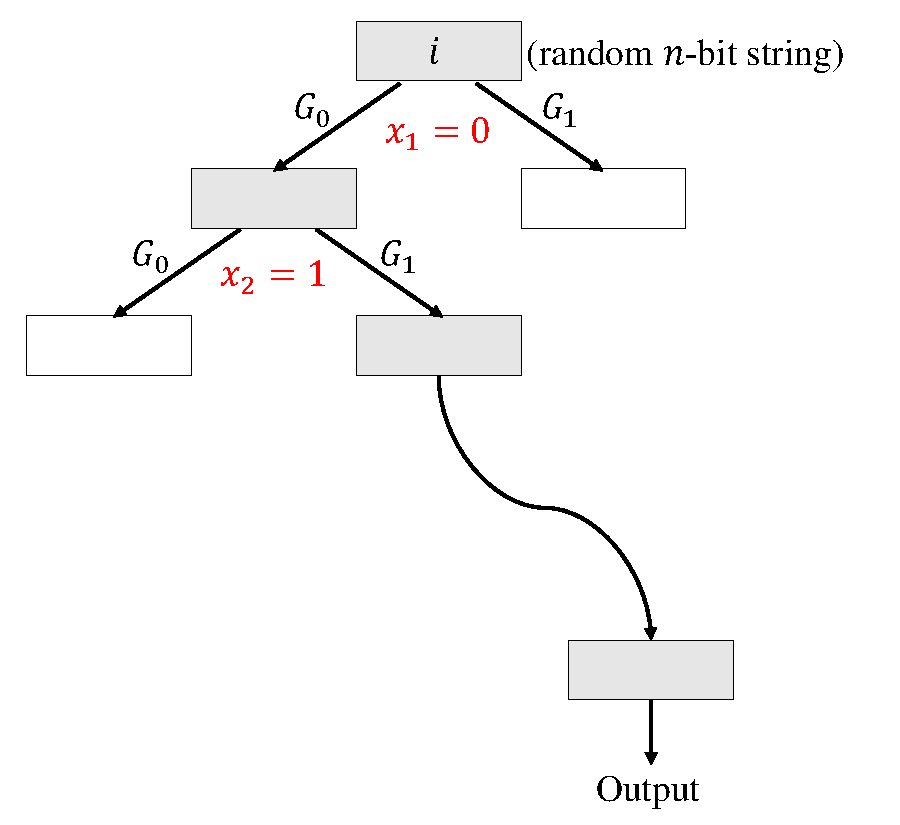
\includegraphics[width=\textwidth]{Old Scribe Notes/binary-tree.pdf}
    \caption{View the construction as a binary tree}
    \label{fig:binary-tree}
\end{marginfigure}

\begin{theorem}\label{theorem:ggm}
The function ensemble $\{F_n\}_{n \in \mathbb{N}}$ constructed above is pseudorandom.
\end{theorem}

\proof
Assume for the sake of contradiction that $\{F_n\}_{n \in \mathbb{N}}$ is not PRG.
Then there exists a non-uniform PPT oracle adversary $\ma$ that can distinguish $\{F_n\}_{n \in \mathbb{N}}$ from $\{R_n\}_{n \in \mathbb{N}}$. Below, via a hybrid argument, we prove that this contradicts the fact that $G$ is a PRG.

Consider the sequence of hybrids $H_i$ for $i \in \{ 0, 1, \cdots, n\}$ where the hybrid $i$ is defined as follows:
\[H_{n,i}^{(K)} (x_1x_2\ldots x_n ):= G_{x_n}(G_{x_{n-1}} (\cdots(G_{x_{i+1}}(K(x_ix_{i-1}\ldots x_1))) \cdots  )), \]
where $K$ is a random function from $\{0,1\}^{i}$ to $\{0,1\}^n$. Intuitively, hybrid $H_i$ corresponds to a binary tree of depth $n$ where the nodes of levels $0$ to $i$ correspond to random values and the nodes at levels $i+1$ to $n$ correspond to pseudorandom values. By inspection, observe that hybrids $H_0$ and $H_n$ are identical to a pseudorandom function and a random function, respectively. There it suffices to prove that hybrids $H_i$ and $H_{i+1}$ are computationally indistinguishable for each $i \in \{ 0, 1, \cdots, n\}$.

We show that $H_{i}$ and $H_{i+1}$ are indistinguishable by considering a sequence of sub-hybrids $H_{i,j}$ for $j \in \{0,\ldots q_{i+1}\}$, where $q_{i+1}$ is the number of the distinct $i-bit$ prefixes of the queries of $\mathcal{A}$.\footnote{Observe that $q_{i+1}$ for each appropriate choice of $i$ is bounded by the running time of $\mathcal{A}$. Hence, this value is bounded by a polynomial in the security parameter.}

We define hybrid $H_{i,j}$ for $j =0$ to be same as hybrid $H_{i}$. Additionally, for $j >0$ hybrid $H_{i,j}$ is defined to be exactly the same as hybrid $H_{i,j-1}$ except the response provided to the attacker for the $j^{th}$ distinct $i-bit$ prefix query of $\mathcal{A}$. Let this prefix be $x^*_n x^*_{n-1} \ldots x^*_{i}$. Note that in hybrid $H_{i,j-1}$ the children of the node $x^*_n x^*_{n-1} \ldots x^*_{i}$ correspond to two pseudorandom values. In hybrid $H_{i,j}$ we replace these two children with random values. By careful inspection, it follows that hybrid $H_{i,q_{i+1}}$ is actually $H_{i+1}$. All we are left to prove is that hybrid $H_{i,j}$ and $H_{i,j+1}$ are indistinguishable for the appropriate choices of $j$ and we prove this below.


Now we are ready to construct an adversary $\mathcal{B}$ that  distinguishes $U_{2n}$ from $G(U_n)$: On input $T \in\{0, 1\}^{2n}$ ($T$ could be either from $U_{2n}$ or $G(U_n)$),
construct a full binary tree of depth $n$ that is exactly the same as $H_{i,j}$ except replacing the children of  $x^*_n x^*_{n-1} \ldots x^*_{i}$ by the value $T$.
Observe that the only difference between $H_{i,j}$ and $H_{i,j+1}$ is that values corresponding to nodes $x_n^*\ldots x_i^* 0$ and $x_n^*\ldots x_i^* 1$ are pseudorandom or random respectively. $\mathcal{B}$ uses the value $T$ to generate these two nodes. Hence success in  distinguishing hybrids $H_{i,j}$ and $H_{i,j+1}$ provides a successful attack for $\mathcal{B}$ in violating security of the pseudorandom generator.
\qed







\section{PRFs from DDH: Naor-Reingold PRF}
We will now describe a PRF function family $F_n: \mathcal{K} \times \{0,1\}^n \rightarrow \mathbb{G}_n$ where DDH is assumed to be hard for  $\{\mathbb{G}_n\}$ and $\mathcal{K}$ is the key space.
The seed for the PRF $F_n$ will be $K =  (h, u_1, \ldots u_n)$, where $u,u_0\ldots u_n$ are sampled uniformly from $|\mathbb{G}_n|$, $g$ is the generator of $\mathbb{G}_n$ and $h = g^u$. 

\[F_n(K,x) = h^{\prod_{i} u_i^{x_i}}\]

Next, we will prove that the function $F_n$ is a pseudo-random function or that $\{F_n\}$ is a pseudo-random function ensemble.\footnote{Here, we require that adversary distinguish the function $F_n$ from a random function from $\{0,1\}^n$ to $\mathbb{G}_n$. Note that the output range of the function is $\mathbb{G}_n$. Note that the distribution of random group elements in $\mathbb{G}_n$ might actually be far from uniformly random strings.}
\begin{lemma}
Assuming the DDH Assumption (see Definition~\ref{def:ddh}) for $\{\mathbb{G}_n\}$ is hard, we have that $\{F_n\}$ is a pseudorandom function ensemble.
\end{lemma}
\begin{proof}
The proof of this lemma is similar to the proof of Theorem~\ref{theorem:ggm}.

Let $R_n^j$ be random function from $\{0,1\}^j \rightarrow \mathbb{G}_n$. Then we want to prove that for all non-uniform PPT adversaries $\mathcal{A}$ we have that:
\[\mu(n) = \left|\Pr[\mathcal{A}^{F_n}(1^n) =1] -  \Pr[\mathcal{A}^{R_n^n}(1^n) =1]\right|\]
is a negligible function. 

For the sake of contradiction, we assume that the function $F_n$ is not pseudorandom. Next, towards a contradiction, we consider a sequence of hybrid functions $F_n^0 \ldots F_n^n$. 
For any $j \in \{0,\ldots n\}$, let $F^j_n((h,u_{j}\ldots u_n),x) = (R_n^j(x_1\ldots x_j))^{\prod_{i=j+1}^n u_i^{x_i}}$, where $R_n^0(\epsilon)$ is the constant function with output $h$. Observe that $F_n^0$ is the same as the function $F_n$ and $F_n^n$ is the same as the function $R_n^n$. Thus, by a hybrid argument, we conclude that there exists $k \in \{0,\ldots n-1\}$, such that 
\[\left|\Pr[\mathcal{A}^{F_n^k}(1^n) =1] -  \Pr[\mathcal{A}^{F_n^{k+1}}(1^n) =1]\right|\]
is a non-negligible function. Now all we are left to show is that this implies an attacker that refutes the DDH assumption. The proof of this claim follows by a sequence of $T$ sub-hybrids, where $T$ is the running time of $\mathcal{A}$. Without loss of generality we assume that $\mathcal{A}$ never makes the same query twice. 

More specifically, we consider a sequence of functions $F_n^{k,t}$ where $t \in \{0,T\}$, $F_n^{k,0}$ is same as $F_n^{k}$ and $F_n^{k,T}$ is same as $F_n^{k+1}$. In particular, we explain how $F_n^{k,t}$ answers queries by $\mathcal{A}$.\footnote{As assumed earlier, keep in mind that $\mathcal{A}$ never makes the same query twice.} Let $x^1, \ldots x^t$ be the first $t$ queries made by $\mathcal{A}$. For any query, $x$ made by $\mathcal{A}$ such that the first $k$ bits of $x$ match the first $k$ bits of one of $x_1, \ldots x_y$ answer as $F_n^{k+1}$ else answer as $F_n^{k}$. Now we can conclude that there exists a $t$ such that $F_n^{k,t}$ and $F_n^{k,t+1}$ are distinguishable with non-negligible probability. 

Finally, we will show that using an adversary that can distinguish between $F_n^{k,t}$ and $F_n^{k,t+1}$ we need to construct an adversary $\mathcal{B}$ that refutes the DDH assumption. We leave construction of this adversary as an exercise.
\end{proof}


\newpage
\section*{Exercises}
\begin{exercise}
\newcommand{\bit}{\{0,1\}}

Prove or disprove: If $f$ is a one-way function, then the following function $B:\bit^*\to\bit$ is a hardconcentrate predicate for $f$. The function $B(x)$ outputs the inner product modulo 2 of the first $\lfloor |x|/2\rfloor$ bits of $x$ and the last $\lfloor |x|/2\rfloor$ bits of $x$.
\end{exercise}

\begin{exercise}
Let $\phi(n)$ denote the first $n$ digits of $\pi = 3.141592653589\ldots$ after the decimal in binary ($\pi$ in its binary notation looks like $11.00100100001111110110101010001000100001\ldots$).

   Prove the following: if one-way functions exist, then there exists a one-way function $f$ such that the function $B:\{0,1\}^* \rightarrow \{0,1\}$ is not a hard concentrate bit of $f$. The function $B(x)$ outputs $\langle x, \phi(|x|)\rangle$, where
    \[\langle a, b\rangle := \sum_{i=1}^n a_i b_i \mod 2\]
    for the bit-representation of $a = {a_1a_2\cdots a_n}$ and $b= {b_1b_2\cdots b_n}$.
\end{exercise}

\begin{exercise}
 If $f: \{0,1\}^{n}\times \{0,1\}^n\rightarrow \{0,1\}^n$  is PRF, then in which of the following cases is $g: \{0,1\}^{n}\times \{0,1\}^n\rightarrow \{0,1\}^n$ also a PRF? \begin{enumerate} \item $g(K,x) = f(K,f(K,x))$ \item $g(K,x) = f(x,f(K,x))$ \item $g(K,x) = f(K,f(x,K))$
    \end{enumerate}
\end{exercise}

\begin{exercise}[Puncturable PRFs.] Puncturable PRFs are PRFs for which a key can be given out such that, it allows evaluation of the PRF on all inputs, except for one designated input.

%\newcommand{\negl}{\mathsf{negl}}
\newcommand{\A}{\mathcal{A}}
\newcommand{\F}{F}
\newcommand{\KeyF}{\mathsf{Key}_{\F}}
\newcommand{\PunctureF}{\mathsf{Puncture}_{\F}}
\newcommand{\EvalF}{\mathsf{Eval}_{\F}}


A puncturable pseudo-random function $\F$ is given by a triple of efficient algorithms ($\KeyF$,$\PunctureF$, and $\EvalF$), satisfying the following conditions:
\begin{itemize}
\item[-] \textbf{Functionality preserved under puncturing}: For every $x^*, x \in \{0,1\}^{n}$ such that $x^* \neq x$, we have that:
    $$\Pr[\EvalF(K,x) = \EvalF(K_{x^*},x) : K \gets \KeyF(1^n), K_{x^*} = \PunctureF(K,x^*)] = 1$$
\item[-] \textbf{Pseudorandom at the punctured point}: For every $x^*\in \{0,1\}^n$ we have that for every polysize adversary $\A$ we have that:
    $$|\Pr[\A(K_{x^*}, \EvalF(K,x^*)) = 1] - \Pr[\A(K_{x^*}, \EvalF(K,U_n)) = 1]|= \negl(n)$$
    where $K \gets \KeyF(1^n)$ and $K_S = \PunctureF(K,x^*)$. $U_n$ denotes the uniform distribution over $n$ bits.
\end{itemize}

Prove that: If one-way functions exist, then there exists a puncturable PRF family that maps $n$ bits to $n$ bits. \\ 
\textbf{Hint:} The GGM tree-based construction of PRFs from a length doubling pseudorandom generator (discussed in class) can be adapted to construct a puncturable PRF. Also note that $K$ and $K_{x^*}$ need not be the same length.
\end{exercise}
%
%\subsection{Application}
%Consider an interesting game: Alice and Bob are talking on the phone.
%Alice flips a coin, and Bob guesses whether it's head or tail.
%But the problem is how can Alice convince Bob that the coin is indeed head or tail?
%If we have pseudorandom functions, the problem could be easily solved.
%
%Assume we have a PRF $F_n: \{0, 1\}^n \rightarrow \{0, 1\}^n$.
%Alice and Bob have a shared key $i \in \{0, 1\}^n$, then $f_i(\cdot)$ is shared information.
%Now Alice has a message $m \in \{0, 1\}^n$ and wants to let Bob guess it,
%the procedure consists of three steps.
%\begin{enumerate}[(a)]
%    \item Alice chooses a string $r \in \{0, 1\}^n$, and sends to Bob  $m' = f_i(r) \oplus m$ ;
%    \item Bob guesses $m$;
%    \item Alice sends $r$ to Bob.
%\end{enumerate}
%In step (a), since $F_n$ is PRF, all the information that Bob gets is a random $n$-bit string, so it will not influence his behavior in step (b).
%Then in step (c), Bob receives $r$ and will be convinced that the true value of $m$ is $f_i(r) \oplus m'$.
%

\chapter{Private-Key Cryptography}
%\newcommand{\key}{\mathsf{k}}
\newcommand{\gen}{\mathsf{Gen}}

\begin{definition}[$\pcnotionstyle{Pri\pcmathhyphen{}}\indcpa$] A private-key encryption scheme $\Pi = (\gen,\enc,\dec)$ is $\pcnotionstyle{Pri\pcmathhyphen{}}\indcpa$-secure if 
$$ \advantage{\indcpa}{\Pi,\adv} = \Large\mid \Pr[\pcnotionstyle{Pri\pcmathhyphen{}}\indcpa_\Pi^\adv(\secpar) =1] -\frac12\Large\mid$$
is a negligible function. 
\end{definition}

\marginnote[-1.5in]{
\procedureblock[linenumbering]{$ \pcnotionstyle{Pri\pcmathhyphen{}}\indcpa_{\Pi}^{\adv}(\secpar)$}{
 b \sample \bin \\
  \key  \sample \gen ( \secparam ) \\
 ( \state ,m_0 ,m_1) \sample \adv^{\enc ( \key ,\cdot )} ( \secparam) \\
 c \sample \enc ( \key ,m_b ) \\
 b' \sample \adv^{\enc ( \key ,\cdot )} ( \state , c ) \\
 \pcreturn b = b' }
 }
\newcommand{\nonnegl}{\mathsf{nonnegl}}


\section{Fixed-length MACs}

Previously, we defined what a MAC is, and specified correctness and security definitions for MACs. In this section, we'll define a fixed-length MAC for length $\ell(n)$.

\begin{theorem}
    If $F : \{0, 1\}^n \to \{0, 1\}^n$ is a PRF, then $\Pi = (\mathsf{Gen}, \mathsf{Mac}, \mathsf{Verify})$ (constructed below) is a MAC, as defined with EF-CMA security.

    \begin{algorithmic}[1]
        \Function{Gen}{$1^n$}
            \State \Return $k \in \{0, 1\}^n$
        \EndFunction
        \Statex
        \Function{Mac}{$k$, $m$}
            \State \Return $F_k(m)$
        \EndFunction
        \Statex
        \Function{Verify}{$k$, $m$, $t$}
            \State \Return $t \overset{?}{=} F_k(m)$
        \EndFunction
    \end{algorithmic}

    That is, we just compute the PRF on our message as the MAC.
\end{theorem}

\begin{proof}
    To prove security, suppose for contradiction that there exists an adversary $A$ that breaks the security for $\Pi$. We'd like to construct an adversary $B$ that breaks the security of the PRF.

    Here, the adversary $A$ expects queries for tags, given messages as input. $B$ can simply forward these requests on to $F$, and return the response back to $A$. Further, $A$ outputs a pair $(m^*, t^*)$, which $B$ can send $m^*$ to $F$, and output whether $t = t^*$.

    \begin{center}
        \begin{tikzpicture}
            \draw (3, 0) rectangle (8, 5.5);
            \draw (5, 0.5) rectangle (7.5, 5);
            \node at (3.25, 5.25) {$B$};
            \node at (5.25, 4.75) {$A$};

            \draw (5.5, 4) edge[->] node[right, pos=0] {$m$} (2.5, 4)
                (2.5, 3.5) edge[->] node[right, pos=1] {$t$} (5.5, 3.5);
            \node[left] at (2.5, 3.75) {$F_k$};
            \node at (5.5, 3.1) {$\vdots$};
            \node at (4.5, 3.1) {$\vdots$};
            \draw (5.5, 2.5) edge[->] node[right, pos=0] {$(m^*, t^*)$} (4.5, 2.5);

            \draw (3.5, 2.5) edge[->] node[right, pos=0] {$m^*$} (2.5, 2.5);
            \node[left] at (2.5, 2.25) {$F_k$};
            \draw (2.5, 2) edge[->] node[right, pos=1] {$t$} (3.5, 2);
            \draw (3.5, 1) edge[->] node[right, pos=0] {$t \overset{?}{=} t^*$} (2.5, 1);
        \end{tikzpicture}
    \end{center}

    Analyzing the probability for $B$, we have
    \[
        \abs{\Pr(B^{F_k(\cdot)}(1^n) = 1) - \Pr(B^{R_n(\cdot)}(1^n) = 1)}
        = \abs{\varepsilon_A(n) - \frac{1}{2^n}}
        = \nonnegl(n)
    .\]
    Here, the first term is because the correctness follows immediately from the correctness of $A$, and the second term is due to the fact that the output of $R_n$ is random.
\end{proof}

\section{Variable-length MACs}

Now, let us look at messages with lengths that are a multiple of $n$. In particular, we have a few blocks $m_1, \ldots, m_{\ell}$, each of size $n$. There are a few ways to do this, but we'll look at a method similar to the counter mode we looked at last time.

\begin{center}
    \begin{tikzpicture}
        \node (m1) at (0, 2) {$m_1$};
        \node (m2) at (1, 2) {$m_2$};
        \node (m3) at (2, 2) {$m_3$};
        \node (mdots) at (3, 2) {$\cdots$};
        \node (ml) at (4, 2) {$m_{\ell}$};

        \node[draw] (fk1) at (0, 0) {$F_k$};
        \node[draw] (fk2) at (1, 0) {$F_k$};
        \node[draw] (fk3) at (2, 0) {$F_k$};
        \node at (3, 0) {$\ldots$};
        \node[draw] (fkl) at (4, 0) {$F_k$};

        \node[outer sep=0pt, inner sep=0pt, draw, circle] (fk1+m2) at (1, 1) {$+$};
        \node[outer sep=0pt, inner sep=0pt, draw, circle] (fk2+m3) at (2, 1) {$+$};
        \node[outer sep=0pt, inner sep=1pt] (xor-dots) at (3, 1) {$\ldots$};
        \node[outer sep=0pt, inner sep=0pt, draw, circle] (dots+ml) at (4, 1) {$+$};

        \draw (m1) edge[->] (fk1)
            (m2) edge[->] (fk1+m2)
            (m3) edge[->] (fk2+m3)
            (ml) edge[->] (dots+ml);

        \draw[->] (fk1) -- ++(0.5, 0) |- (fk1+m2);
        \draw[->] (fk2) -- ++(0.5, 0) |- (fk2+m3);
        \draw[->] (fk3) -- ++(0.5, 0) |- (xor-dots);

        \draw[->] (xor-dots) -- (dots+ml);
        \draw (fk1+m2) edge[->] (fk2)
            (fk2+m3) edge[->] (fk3)
            (dots+ml) edge[->] (fkl);
        \draw (fkl) edge[->] ++(1, 0);
    \end{tikzpicture}
\end{center}

This construction avoids having to store a tag equal in length to the message, but this is not secure, due to length extension attacks. In particular, suppose we query for the tag $t$ associated with $0^n$. We can then query another tag $t'$ for $0^n \oplus t$. Observe here that $t'$ is also the tag for $0^{2n}$.

A solution is to use different keys for each PRF, but this isn't too efficient, since we're still calling the PRF once per block of length $n$. We'll instead improve this to use only one block cipher call---we do some preprocessing and only call $F_k$ once on the output of the preprocessing.

In particular, we'll claim that applying a universal hash function to the input and then applying the block cipher is a secure MAC.

\begin{definition}[Universal Hash Function]
    A function $h : \mathcal{F} \times \mathcal{F}^* \to \mathcal{F}$ (where $\mathcal{F}$ is a field of size $2^m$) is a universal hash function if for all $m, m' \in \mathcal{F}^{\le \ell}$ (i.e. $m$ and $m'$ have length at most $\ell$),
    \[
        \Pr_s(h(s, m) = h(s, m')) \le \frac{\ell}{\abs{F}}
    .\]
    That is, the probability of collision is small.
\end{definition}

Crucially here, we fix $m$ and $m'$, and we sample $s$. (If we fix an $s$, we can almost surely find an $m$ and $m'$ that collide.)

Today, we'll look at the following function:
\[
    h(s, m_0, \ldots, m_{\ell - 1}) = m_0 + m_1 s + m_2 s^2 + \cdots + m_{\ell - 1} s^{\ell - 1} + s^{\ell}
.\]

\begin{claim}
    The function defined by
    \[
        h(s, m_0, \ldots, m_{\ell - 1}) = m_0 + m_1 s + m_2 s^2 + \cdots + m_{\ell - 1} s^{\ell - 1} + s^{\ell}
    \]
    is a universal hash function.
\end{claim}

\begin{proof}
    We'd like to argue that for a fixed $m$ and $m'$, and a random $s$, the probability that there is a collision is at most $\frac{\ell}{\abs{\mathcal{F}}}$.

    We'll look at
    \[
        h(x, m_0, \ldots, m_t) - h(x, m_0', \ldots, m_t') = (m_0 - m_0') + \cdots + (m_{t - 1} - m_{t-1}') x^{\ell - 1}
    .\]
    If there is a collision, this difference is 0. The probability that this polynomial of degree at most $\ell$ has a zero at $x$ is at most $\frac{\ell}{\abs{\mathcal{F}}}$, since it has at most $\ell$ zeroes. This means that $h$ is indeed a universal hash function.
\end{proof}

\begin{claim}
    The MAC given by $F_k(h(s, m_1, \ldots, m_{\ell}))$, for the universal hash function $h$ given prior, is secure. (This is a slight variation on the Carter--Wegman MAC.)
\end{claim}

\begin{proof}
    Suppose for contradiction that there exists a nu-PPT $A$ that breaks the security of this scheme.

    Here, for appropriately generated $k$ and $s$, $A$ makes queries $m \mapsto F_k(h_s(m))$, and outputs $(m^*, t^*)$.

    We'd like to create an adversary $B$ that either breaks the security of the PRF, or breaks the security of the universal hash function.

    $B$ will start by sampling $s \in \mathcal{F}$. When given the query for $m_1$, it computes $h_s(m_1)$ and queries for $F_k(h_s(m_1))$, which it sends back to $A$. If $F_k$ was actually pseudorandom, then $A$ is given a pseudorandom input, and if $F_k$ was random $R_n$, then $A$ is given a random input.

    $A$ must still be able to generate pairs $(m^*, t^*)$ even when given a random input, due to the security of the PRF.

    \begin{center}
        \begin{tikzpicture}
            \draw (2, 0) rectangle (8, 5.5);
            \draw (5, 0.5) rectangle (7.5, 5);
            \node at (2.25, 5.25) {$B$};
            \node at (5.25, 4.75) {$A$};

            \node at (3.5, 4.5) {sample $s \in \mathcal{F}$};

            \node (hsm) at (3.5, 4) {$h_s(m)$};
            \draw (5.5, 4) edge[->] node[right, pos=0] {$m$} (hsm)
                (hsm) edge[->] (1.5, 4)
                (1.5, 3.5) edge[->] node[right, pos=1] {$t$} (5.5, 3.5);
            \node[left] at (1.5, 3.75) {$F_k$};
            \node at (5.5, 3.1) {$\vdots$};
            \node at (4.5, 3.1) {$\vdots$};

            \node (hash-m-star) at (3.5, 2.5) {$h_s(m^*)$};
            \draw (5.5, 2.5) edge[->] node[right, pos=0] {$(m^*, t^*)$} (hash-m-star)
                (hash-m-star) edge[->] (1.5, 2.5);
            \node[left] at (1.5, 2.25) {$F_k$};
            \draw (1.5, 2) edge[->] node[right, pos=1] {$t$} (3.5, 2);
            \draw (3.5, 1) edge[->] node[right, pos=0] {$t \overset{?}{=} t^*$} (1.5, 1);
        \end{tikzpicture}
    \end{center}

    Let $E$ be the event that there exists an $m, m' \in L \cup \{m^*\}$, such that $h_s(m) = h(m')$. If $E$ does not happen, then the hash function never collides. This means that the attacker only sees random values depending on distinct inputs, so this reduces to the case from earlier (when the MAC is just $F_k$).

    As such, we'd like to show that collisions in $h_s(\cdot)$ occur with negligible probability.

    To show this, suppose for contradiction that collisions actually do occur with non-negligible probability. We then want to construct an adversary $B$ utilizing $A$ that just outputs $m$ and $m'$ such that when $s$ is sampled, $h_s(m) = h_s(m')$ with high probability.

    $B$ will pick a random $i, j \in \{1, \ldots, q+1\}$ (here suppose $i < j$), where $q$ is the number of MAC queries. We then run $A$ until the $j$th query. Taking the $i$th and $j$th query, we then output $m_i$ and $m_j$ as our pair of messages. We still need to entertain the queries made by $A$, so we can just return random values for tags (giving the same value if it requests it for the same message).

    \begin{center}
        \begin{tikzpicture}
            \draw (2, 0) rectangle (8, 6);
            \draw (5, 0.5) rectangle (7.5, 5.5);
            \node at (2.25, 5.75) {$B$};
            \node at (5.25, 5.25) {$A$};

            \node[align=center] at (3.5, 5) {\small $i, j \xleftarrow{\$} \{1, \ldots, q+1\}$};

            \draw (5.5, 4) edge[->] node[right, pos=0] {$m_1$} (4.5, 4)
                (4.5, 3.5) edge[->] node[left, pos=0] {sample $t_1$} node[right, pos=1] {$t_1$} (5.5, 3.5);
            \node at (5.5, 3.1) {$\vdots$};
            \node at (4.5, 3.1) {$\vdots$};

            \draw (5.5, 2.5) edge[->] node[right, pos=0] {$m_i$} (4.5, 2.5)
                (4.5, 2) edge[->] node[left, pos=0] {sample $t_i$} node[right, pos=1] {$t_i$} (5.5, 2);
            \node at (5.5, 1.6) {$\vdots$};
            \node at (4.5, 1.6) {$\vdots$};

            \draw (5.5, 1) edge[->] node[right, pos=0] {$m_j$} (4.5, 1);

            \draw (3, 0.5) edge[->] node[right, pos=0] {$(m_i, m_j)$} (1.5, 0.5);
        \end{tikzpicture}
    \end{center}

    By assumption, we know that $E$ occurs with non-negligible probability. That is, among the queries made by $A$, there is a non-negligible probability that $h_s(m_i) = h_s(m_j)$. Since here the implementation of $B$ just picks out a pair of random queries from those made by $A$, the pair $(m_i, m_j)$ output by $B$ also has a collision with non-negligible probability. (In particular, with probability $\Pr(E) / q^2$.

    This breaks the definition of a universal hash function, which is a contradiction.
\end{proof}

So far, we know how to generate tags of fixed length, and of lengths that are a multiple of $n$. If we have a message that is not a multiple of $n$, we could potentially just pad the input with 0's, but this causes an issue, as $m$ and $m \concat 0$ have the same tag.

Instead, one solution is to put the size of the message in the first block, and we can still put the padding at the end. This way, if the messages differ by length, the first block will be different, and if the messages do not differ by length, then we're essentially just ignoring the padding. This gives us a MAC for arbitrary-length messages.

\section{Authenticated Encryption Schemes}

We've talked about confidentiality and integrity separately, but generally we want both properties---when Alice sends a message to Bob, we'd like for any eavesdropper to be unable to recover the message, \emph{and} we'd like Bob to be able to verify that the message actually came from Alice.

A scheme that achieves both of these conditions is called an \emph{authenticated encryption scheme}.

\begin{definition}[Authenticated Encryption Scheme]
    A scheme $\Pi$ is an \emph{authenticated encryption scheme} if it is CPA-secure, and it has ciphertext integrity (CI).
\end{definition}

\begin{definition}[Ciphertext Integrity (CI)]
    Consider the following game for the scheme $\Pi = (\mathsf{Gen}, \mathsf{Enc}, \mathsf{Dec})$.

    \begin{algorithmic}[1]
        \Function{CI${}_{\Pi}^A$}{$n$}
            \State $k \gets \mathsf{Gen}(1^n)$
            \State $c^* \gets A^{\mathsf{Enc}(k, \cdot)}(1^n)$
            \State $L \gets$ the list of queries made by $A$
            \State \Return $(\mathsf{Dec}(k, c^*) \ne \bot) \land (c^* \notin L)$
        \EndFunction
    \end{algorithmic}

    A scheme has ciphertext integrity if for all nu-PPT $A$, $\Pr(\mathrm{CI}_{\Pi}^A)$ is negligible.
\end{definition}

Observe that an authenticated encryption scheme is also CCA-secure, since the CI property says that the adversary can never generate a valid ciphertext. This means that whenever an adversary requests the decryption of a ciphertext, we can always return $\bot$ (unless they previously requested a ciphertext for a message, and wants to decode that ciphertext). This means that the decryption oracle is essentially useless, and this reduces to the CPA case.

Next, we'll construct an authenticated encryption scheme, called ``Encrypt-then-MAC'', utilizing a CPA-secure encryption scheme and an EF-CMA MAC scheme.

\begin{claim}
    Let $\Pi_e = (\mathsf{Gen}_e, \mathsf{Enc}_e, \mathsf{Dec}_e)$ be a CPA-secure encryption scheme, and let $\Pi_m = (\mathsf{Gen}_m, \mathsf{Mac}_m, \mathsf{Verify}_m)$ be an EF-CMA-secure MAC scheme.

    The following scheme $\Pi = (\mathsf{Gen}, \mathsf{Enc}, \mathsf{Dec})$ is an authenticated encryption scheme.

    \begin{algorithmic}[1]
        \Function{Gen}{$1^n$}
            \State $k_e \gets \mathsf{Gen}_e(1^n)$
            \State $k_m \gets \mathsf{Gen}_m(1^n)$
            \State \Return $(k_e, k_m)$
        \EndFunction
        \Statex
        \Function{Enc}{$(k_e, k_m), m$}
            \State $c \gets \mathsf{Enc}_e(k_e, m)$
            \State $t \gets \mathsf{Mac}_m(k_m, c)$
            \State \Return $(c, t)$
        \EndFunction
        \Statex
        \Function{Dec}{$(k_e, k_m), (c, t), m$}
            \If {$\mathsf{Verify}_m(k_m, c, t)$}
                \State \Return $\mathsf{Dec}_e(k_e, c)$
            \Else
                \State \Return $\bot$
            \EndIf 
        \EndFunction
    \end{algorithmic}
\end{claim}

\begin{proof}
    Suppose for contradiction that we have an adversary $A$ that breaks the CPA security of $\Pi$. The CPA game allows for queries of the ciphertext for messages $m$, produces a pair $m_0, m_1$, and then gets $c^* = \mathsf{Enc}(k, m_B)$, and $A$ eventually outputs $b'$ to identify which message was encrypted.

    We'd like to construct another adversary $B$, which breaks the CPA-security of $\Pi_e$. The only difference here is the MACs, so $B$ can sample a $k_m \gets \mathsf{Gen}_m(1^n)$, and perform all of the MACs itself.

    In particular, when $A$ asks for the ciphertext of $M$, we pass it to the oracle for $\Pi_e$, and attach $t \gets \mathsf{Mac}_m(k_m, c)$. If $A$ is able to distinguish between ciphertexts of $M_0$ and $M_1$, then we can use the same bit to distinguish between ciphertexts for $\Pi_e$.
    \begin{center}
        \begin{tikzpicture}
            \draw (1.5, -1) rectangle (8, 6);
            \draw (5, -0.5) rectangle (7.5, 5.5);
            \node at (1.75, 5.75) {$B$};
            \node at (5.25, 5.25) {$A$};

            \node at (3.25, 5) {$k_m \gets \textsc{Gen}_m(1^n)$};

            \node (enc) at (3.25, 3.5) {$C = \textsc{Enc}_e(k_e, m)$};
            \node (mac) at (3.25, 3) {$(C, \textsc{Mac}_m(k_m, C))$};

            \draw (5.5, 4) edge[->] node[right, pos=0] {$m$} (1, 4)
                (1, 3.5) edge[->] (enc)
                (mac) edge[->] node[right, pos=1] {$c$} (5.5, 3);
            \node[left] at (1, 3.75) {$\textsc{Enc}_e(k_e, \cdot)$};
            \node at (5.5, 2.6) {$\vdots$};
            \node at (4.5, 2.6) {$\vdots$};

            \draw (5.5, 2) edge[->] node[right, pos=0] {$m_1, m_2$} node[left, pos=1] {$m_1, m_2$} (1, 2);
            \node (enc-mb) at (3.25, 1.5) {$C^*$};
            \node (mac-mb) at (3.25, 1) {$(C^*, \textsc{Mac}_m(k_m, C^*))$};
            \draw (1, 1.5) edge[->] node[left, pos=0] {$\textsc{Enc}_e(k_e, m_b)$} (enc-mb);
            \draw (mac-mb) edge[->] node[right, pos=1] {$c^*$} (5.5, 1);

            \node at (5.5, 0.5) {$\vdots$};
            \node at (4.5, 0.5) {$\vdots$};

            \draw (5.5, 0) edge[->] node[right, pos=0] {$b'$} (1, 0);
        \end{tikzpicture}
    \end{center}

    To prove ciphertext integrity, suppose we have an adversary $A$ that breaks the ciphertext integrity of $\Pi$. Here, $A$ asks for ciphertext queries, and eventually returns a new ciphertext that is valid.

    We'd like to construct an adversary $B$ that is able to generate a new message and a tag, given oracle access to the MAC scheme. The construction will follow similarly to the prior proof on CPA security.

    Here, our adversary $B$ can sample $k_e \gets \mathsf{Gen}_e(1^n)$. When $A$ asks for the encryption of $M$, $B$ can send $m = \mathsf{Enc}_e(k_e, M)$ to the MAC oracle, and it returns $c = (m, t)$ to $A$.

    When $A$ returns $C^* = (c^*, t^*)$, $B$ can also just return the same, since the tag $t^*$ is being computed on $c^*$.

    \begin{center}
        \begin{tikzpicture}
            \draw (1.5, 1) rectangle (8, 6);
            \draw (5, 1.5) rectangle (7.5, 5.5);
            \node at (1.75, 5.75) {$B$};
            \node at (5.25, 5.25) {$A$};

            \node at (3.25, 5) {$k_e \gets \textsc{Gen}_e(1^n)$};

            \node (enc) at (3.25, 4) {$C = \textsc{Enc}_e(k_e, m)$};
            \node (mac) at (3.25, 3.5) {$T = \textsc{Mac}_m(k_m, C)$};
            \node (enc-mac) at (3.25, 3) {$(C, T)$};

            \draw (5.5, 4) edge[->] node[right, pos=0] {$m$} (enc)
                (enc) edge[->] (1, 4)
                (1, 3.5) edge[->] (mac)
                (enc-mac) edge[->] node[right, pos=1] {$c$} (5.5, 3);
            \node[left] at (1, 3.75) {$\textsc{Mac}_m(k_m, \cdot)$};
            \node at (5.5, 2.6) {$\vdots$};
            \node at (4.5, 2.6) {$\vdots$};

            \node (gen-ciphertext) at (3.25, 2) {$(C^*, T^*)$};
            \draw (5.5, 2) edge[->] node[right, pos=0] {$c^*$} (gen-ciphertext)
                (gen-ciphertext) edge[->] (1, 2);
        \end{tikzpicture}
    \end{center}
\end{proof}

As an example, AES-GCM is the most popular authenticated encryption scheme that is used, and also has the ability to authenticate additional data. (AES-GCM basically just appends the associated data to the ciphertext, so that the encryption is only on the message, but the MAC is on both the ciphertext and the associated data.) This scheme uses a counter-mode encryption scheme, and the MAC that we saw, but makes this more efficient.


% !TEX root = collection.tex

\chapter{Digital Signatures}

In this chapter, we will introduce the notion of a digital signature. At an intuitive level, a digital signature scheme helps providing authenticity of messages and ensuring non-repudiation. We will first define this primitive and then construct what is called as one-time secure digital signature scheme. An one-time digital signature satisfies a weaker security property when compared to digital signatures. We then introduce the concept of collision-resistant hash functions and then use this along with a one-time secure digital signature to give a construction of digital signature scheme.

\section{Definition}

A digital signature scheme is a tuple of three algorithms $(\Gen,\Sign,\Verify)$ with the following syntax:
\begin{enumerate}
\item $\Gen(1^n)\to (vk,sk)$: On input the message length (in unary) $1^n$, $\Gen$ outputs a secret signing key $sk$ and a public verification key $vk$.
\item $\Sign(sk, m) \to \sigma$: On input a secret key $sk$ and a message $m$ of length $n$, the $\Sign$ algorithm outputs a signature $\sigma$.
\item $\Verify(vk, m, \sigma) \to \{0,1\}$: On input the verification key $vk$, a message $m$ and a signature $\sigma$, the $\Verify$ algorithm outputs either $0$ or $1$.
\end{enumerate}

We require that the digital signature to satisfy the following correctness and security properties.\\
\medskip
\noindent\textbf{Correctness.} For the correctness of the scheme, we have that
$\forall m \in \bin^n$,
\[\Pr \left[ (vk,sk) \gets \Gen(1^n), \sigma \leftarrow \Sign(sk,m) : \Verify(vk, m, \sigma) = 1 \right] = 1.\]

\medskip
\noindent\textbf{Security.} Consider the following game between an adversary and a challenger
.

\begin{enumerate}
    \item The challenger first samples $(vk,sk) \gets \Gen(1^n)$. The challenger gives $vk$ to the adversary.
    \item \textbf{Signing Oracle.} The adversary is now given access to a signing oracle. When the adversary gives a query $m$ to the oracle, it gets back $\sigma \gets \Sign(sk,m)$.
    \item \textbf{Forgery.} The adversary outputs a message, signature pair $(m^*,\sigma^*)$ where $m^*$ is different from the queries that adversary has made to the signing oracle.
    \item The adversary wins the game if $\Verify(vk,m^*,\sigma^*) = 1$.
\end{enumerate}
We say that the digital signature scheme is secure if the probability that the adversary wins the game is $\negl(n)$.

\section{One-time Digital Signature}
\label{lampart}
An one-time digital signature has the same syntax and correctness requirement as that of a digital signature scheme except that in the security game the adversary is allowed to call the signing oracle only once (hence the name one-time). We will now give a construction of one-time signature scheme from the assumption that one-way functions exists.

Let $f: \bin^n \rightarrow \bin^n$ be a one-way function.
\begin{itemize}
\item $\Gen(1^n)$: On input the message length (in unary) $1^n$, $\Gen$ does the following:
\begin{enumerate}
    \item Chooses $x_{i,b} \gets \bin^n$ for each $i \in [n]$ and $b \in \bin$.
    \item Output $vk = \left[ \begin{array}{ccc}
f(x_{1,0}) & \ldots & f(x_{n,0}) \\
f(x_{1,1}) & \ldots & f(x_{n,1}) \\
\end{array} \right]$ and $sk = \left[ \begin{array}{ccc}
x_{1,0} & \ldots & x_{n,0} \\
x_{1,1} & \ldots & x_{n,1} \\
\end{array} \right]$
\end{enumerate}
\item $\Sign(sk, m)$: On input a secret key $sk$ and a message $m \in \bin^n$, the $\Sign$ algorithm outputs a signature $\sigma = x_{1,m_1}\|x_{2,m_2}\| \ldots \| x_{n,m_n}$.
\item $\Verify(vk, m, \sigma)$: On input the verification key $vk$, a message $m$ and a signature $\sigma$, the $\Verify$ algorithm does the following:
\begin{enumerate}
    \item Parse $\sigma = x_{1,m_1}\|x_{2,m_2}\| \ldots \| x_{n,m_n}$.
    \item Compute $vk'_{i,m_i} = f(x_{i,m_i})$ for each $i \in [n]$.
    \item Check if for each $i \in [n]$, $vk'_{i,m_i} = vk_{i,m_i}$. If all the checks pass, output 1. Else, output 0.
\end{enumerate}
\end{itemize}

Before we prove any security property, we first observe that this scheme is completely broken if we allow the adversary to ask for two signatures. This is because the adversary can query for the signatures on $0^n$ and $1^n$ respectively and the adversary gets the entire secret key. The adversary can then use this secret key to sign on any message and break the security. 

We will now argue the one-time security of this construction. Let $\adv$ be an adversary who breaks the security of our one-time digital signature scheme with non-negligible probability $\mu(n)$. We will now construct an adversary $\advb$ that breaks the one-wayness of $f$. $\advb$ receives a one-way function challenge $y$ and does the following:
\begin{enumerate}
    \item $\advb$ chooses $i^*$ uniformly at random from $[n]$ and $b^*$ uniformly at random from $\bin$.
    \item It sets $vk_{i^*,b^*} = y$
    \item For all $i \in [n]$ and $b \in \bin$ such that $(i,b) \neq (i^*,b^*)$, $\advb$ samples $x_{i,b} \gets \bin^n$. It computes $vk_{i,b} = f(x_{i,b})$.
    \item It sets $vk = \left[ \begin{array}{ccc}
vk_{1,0} & \ldots& vk_{n,0} \\
vk_{1,1} & \ldots& vk_{n,1} \\
\end{array} \right]$ and sends $vk$ to $\adv$.
\item $\adv$ now asks for a signing query on a message $m$. If $m_{i^*} = b^*$ then $\advb$ aborts and outputs a special symbol $\abort_1$. Otherwise, it uses it knowledge of $x_{i,b}$ for $(i,b) \neq (i^*,b^*)$ to output a signature on $m$.
\item $\adv$ outputs a valid forgery $(m^*,\sigma^*)$. If $m^*_{i^*} = m_{i^*}$ then $\advb$ aborts and outputs a special symbol $\abort_2$. If it does not abort, then it parses $\sigma^*$ as ${1,m_1}\|x_{2,m_2}\| \ldots \| x_{n,m_n}$ and outputs $x_{i^*,b^*}$ as the inverse of $y$.
\end{enumerate}
We first note that conditioned on $\advb$ not outputting $\abort_1$ or $\abort_2$, the probability that $\advb$ outputs a valid preimage of $y$ is $\mu(n)$. Now, probability $\advb$ does not output $\abort_1$ or $\abort_2$ is $1/2n$ (this is because $\abort_1$ is not output with probability $1/2$ and conditioned on not outputting $\abort_1$, $\abort_2$ is not output with probability $1/n$). Thus, $\advb$ outputs a valid preimage with probability $\mu(n)/2n$. This completes the proof of security.

We now try to extend this one-time signature scheme to digital signatures. For this purpose, we will rely on a primitive called as collision-resistant hash functions.

\section{Universal One-way Hash Function -- UOWHF}
We now introduce a class of hash function called universal one-way hash function. 
This form of hash function is stronger than the universal hash function in 4.10 in the sense that the attacker is allowed to select the input by itself but must do so before being presented with the functions description. 

\subsection{Definition}
We now give a formal definition of universal one-way hash function(UOWHF, also called "WOOF"). 
\begin{definition}[Universal One-way Hash Function(UOWHF)]
    Let $\ell$: $\mathbb{N}\rightarrow\mathbb{N}$. A \textit{collection of functions} 
    $\{h_s: \bit^*\rightarrow\bit^{\ell(|s|)}\}_{s\in\bit^{*}}$ is called universal one-way hash functions given $\exists$ PPT machine $I$ such that: 
    \begin{enumerate}
        \item (Easy to compute): $\exists$ a deterministic machine $M$ such that $M(s,x)=h_s(x)$.
        \item (Hard to form designated collisions): Given a PPT attacker $\mathcal{A}$, the probability of $\mathcal{A}$ to win WOOF game is negligible. 
        \[
            \Pr[WOOF^{I,h}_{\mathcal{A}}(n)=1]=\negl
        \]
    \end{enumerate}
\end{definition}
Where $WOOF^{I,h}_{\mathcal{A}}$ is defined in the following:
\begin{enumerate}
    \item $(state, x)\leftarrow\mathcal{A}(1^n)$.
    \item $s\leftarrow I(1^n)$.
    \item $y\leftarrow\mathcal{A}(state, s)$
    \item Output $h_s(x)=h_s(y)$
\end{enumerate}


\subsection{Construction}
We construct UOWHF collections in several steps, starting with a related but
restricted notion and relaxing the restriction gradually until we reach the unrestricted notion of UOWHF collections. 

\begin{definition}[$(d,r)$-UOWHFs]
Let $d,r$: $\mathbb{N}\rightarrow\mathbb{N}$. A \textit{collection of functions} 
    $\{h_s: \bit^{(d(|s|))}\rightarrow\bit^{r(|s|)}\}_{s\in\bit^{*}}$ is called  $(d,r)$-UOWHFs given $\exists$ PPT machine $I$ such that: 
    \begin{enumerate}
        \item $\exists$ a deterministic machine $M$ such that given $s$ and $x\in\bit^{(d(|s|))}$, $M(s,x)=h_s(x)$.
        \item (Hard to form designated collisions): Given a PPT attacker $\mathcal{A}$, the probability of $\mathcal{A}$ to win WOOF game is negligible. 
        \[
            \Pr[WOOF^{I,h}_{\mathcal{A}}(n)=1]=\negl
        \]
    \end{enumerate}
\end{definition}
And $d,r$ satisfying $d(n)>r(n)$. The other case is trivial to discuss. 

Now we discuss the construction of $4$ types of UOWHFs. We start from the simple cases and eventually lead to the full-fledged UOWHFs.

\noindent\textbf{Step I: $(d, d-1)$-UOWHFs}.
We construct UOWHFs that given arbitrary length, truncate its input length by 1. 
\begin{construction}
    Let $f$: $\bit^{*}\rightarrow\bit^{*}$ be a one-way permutation, and $a,b\in GF(2^n)$. We construct $h_s: \bit^{n}\rightarrow\bit^{n-1}$: 
    \[
        h_{s=(a,b)}(x)=chop(a\cdot f(x)+b)
    \]
    where $chop(\cdot)$ is the function that chops the first bit of a given bit string. 
\end{construction}
We then argue that $h_s$ is a $(d,d-1)$-UOWHF. 

\begin{proof}
    We prove this by contradiction. If an adversary $\mathcal{A}$ can break the security of UOWHF, we can construct an adversary $\mathcal{B}$ that breaks the OWF $f$. 

    The algorithm of $\mathcal{B}$ is as follows upon receive an input $y$:
    \begin{enumerate}
        \item $\mathcal{A}$ first emits the preimage $x_0$ of its chosen.
        \item Attacker $\mathcal{B}$ compute $s=(a,b)$ such that $h_s(y)=h_s(x_0)$.
        \item Input $s=(a,b)$ to the oracle $\mathcal{A}$ and output what $\mathcal{A}$ outputs. 
    \end{enumerate}
    
    Since $h_s$ works by chopping the first bit of $af(x)+b$, there are two elements in the preimage of $h_s(x)$, namely $x$ and $x'=f^{-1}(y)$. 
    Because it is easy to compute $a$ and $b$ that $af(x)+b=ay+b$, the hardness relies on finding $x'$ given $y$, which is inverting the one-way permutation. 
    This creates a contradiction of one-way permutation. 
\end{proof}

\noindent\textbf{Step II: $(2n, n)$-UOWHFs}.
Now we construct length-restricted UOWHFs that shrink their input by a factor of 2.

\begin{construction}
    Let $\{h_s: \bit^{*}\rightarrow\bit^{*-1}\}_{s\in\bit^{*}}$. We construct $H_{s_1\cdots s_n}:\bit^{2n}\rightarrow\bit^{n}$:
    \[
        H_{s_1\cdots s_n}=h_{s_1}^{n+1,n}(h_{s_2}^{n+2,n+1}(\cdots h_{s_n}^{2n,2n-1}(x))\cdots)
    \]
\end{construction}
We now prove that $H$ is a $(2n, n)$-UOWHF given $h$ is a $(d,d-1)$-UOWHF.
That is, if we have an attacker $\mathcal{A}$ that can break $(2n, n)$-UOWHF, we can construct an attacker $\mathcal{B}$ that can break the $(d,d-1)$-UOWHF. 
Our intuition is that the attacker $\mathcal{B}$ can randomly inject the challenge $s_i$ into a random location of $S$ to $\mathcal{A}$ and $\mathcal{A}$ will have a non-negligible probability to create a collision. 

\begin{proof}
    Formally we define the procedure of $\mathcal{B}$:
    \begin{enumerate}
        \item Select $i\in [n]$.
        \item $\forall i'\neq i$, sample $s_{i'}$.
        \item Receive $x_0$ from $\mathcal{A}$.
        \item Compute $x_i^0 = H_{partial}(x_0)=h_{s_{n-i+1}}^{2n-i+1,2n-i}(\dots(h_{s_n}^{2n,2n-1}(x))\dots)$, which is the input of i-th hash round select by $\mathcal{B}$
        \item Output $x_0$ to the challenger.
        \item Receive $S_{i}$ from the challenger. And send $\{S_0,\dots,S_n\}$ to $\mathcal{A}$.
        \item $\mathcal{A}$ output $x_1$.
        \item $\mathcal{B}$ compute $H_{partial}(x_1)$ and output.
    \end{enumerate}

The core idea is that if $\mathcal{A}$ can output a collision with different $x$, the output will be the same at some point in the hash chain of applying $h$. 
Therefore $\mathcal{B}$ can randomly insert the challenge into $\mathcal{A}$.
And with $\mu(\mathcal{A})/n$ probability $\mathcal{B}$ will succeed.  $\mu(\mathcal{A})$ is the probability that $\mathcal{A}$ succeed. 
\end{proof}

\noindent\textbf{Step III: UOWHFs that shrinks any input by a factor of two}.

\begin{construction}[(a $(2n^{*}, n^{*})$-UOWHF for any length of $n^{*}$)]
    Let $\{h_s:\bit^{2n}\rightarrow\bit^{n}\}_{s\in\bit^{*}}$. Then for every $x\in\bit^{*}$ we have
    \[
    H_s(x)=h_s(x_1)\cdots h_s(x_{t}10^{n^{*}-|x_t|-1})
    \]
    where $x=x_1\cdots x_t$, $0\leq|x_t|\leq n^{*}$ and $|x_i|=n^{*}$ for $i=1,\dots,t-1$.
\end{construction}

We now give the proof sketch here. 
We want to prove that $H$ is a $(2n^{*}, n^{*})$-UOWHF given $h$ is a $(2n, n)$-UOWHF.
Because $H_s(x)$ is just parallelize $(2n, n)$-UOWHF multiple times. 

We assume that $\mathcal{A}$ is able to create a collision $x'$ for some input $x$ of its given and $s$.
Some block $x'_i$ will be different than the block $x_i$. 
Therefore we have $h_s(x'_i)=h_s(x_i)$ which create contradiction of $h$ is a $(2n, n)$-UOWHF.

\noindent\textbf{Step IV: Full-Fledged UOWHFs}. 
The last step on our way consists of using UOWHFs as constructed in Step III above to obtain
full-fledged UOWHFs.
\begin{construction}[(a UOWHF)]
Let $\{h_s:\bit^{*}\rightarrow\bit^{*}\}_{s\in\bit^{*}}$, such that $|h_s(s)|=|x|/2$, for every $x\in\bit^{2i\cdot|s|}$ where $i\in\mathbb{N}$. Then for every $s_a,\cdots,s_n\in\bit^{n}$, every $t\in\mathbb{N}$ and $x\in\bit^{2^t\cdot n}$, we define
\[
    H_{s_1,\dots,s_n}(x)=(t,h_{s_t}(\cdots(h_{s_2}(h_{s_1}(x)))\cdots))
\]
\end{construction}
The proof is similar in Step II. 

We show how to use the arbitrary-length WOOF we constructed to boost this one-time, fixed-length digital signature scheme into a one-time, arbitrary-length digital signature scheme. 

\subsection{Removing Length-Restriction from One-Time Digital Signatures} 

Let $(\Gen_\ell, \Sign_\ell, \Verify_\ell)$ be a length-restricted one-time digital signature for messages of length $\ell(n)$. 
Let $h_s: \{0,1\}^* \to \{0,1\}^n$ be a WOOF. 
First we will review an \emph{insecure} first attempt at a construction for $\ell(n) = n$: 
\begin{itemize}
    \item $\Gen^{\text{BAD}}(1^n)$: Run $(pk_\ell, sk_\ell) \leftarrow \Gen_\ell(1^n)$, $s \leftarrow I(1^n)$. Output $((pk_\ell,s),sk_\ell)$.

    \item $\Sign^{\text{BAD}}(sk=sk_\ell, m)$: Output $\Sign_\ell(sk_\ell, h_s(m))$. 

    \item $\Verify^{\text{BAD}}(pk=(pk_\ell,s), m, \sigma)$: Output $\Verify_\ell(pk_\ell, h_s(m), \sigma)$. 
\end{itemize}
Notice that this construction does not work because the seed for the WOOF is revealed before the message is chosen, in which case WOOF security does not apply. 

To avoid this, we can use the following construction for $\ell(n) = k(n) + n$ where $k(n)$ is the length of the seed produced by $I(1^n)$: 
\begin{itemize}
    \item $\Gen(1^n)$: Run $(pk_\ell, sk_\ell) \leftarrow \Gen_\ell(1^n)$. Output $(pk_\ell,sk_\ell)$.

    \item $\Sign(sk=sk_\ell, m)$: Run $s \leftarrow I(1^n)$ and $\sigma_\ell \leftarrow \Sign_\ell(sk_\ell, s || h_s(m))$. Output $(\sigma_\ell, s)$. 

    \item $\Verify(pk=pk_\ell, m, \sigma = (\sigma_\ell, s))$: Output $\Verify_\ell(pk_\ell, s || h_s(m), \sigma_\ell)$. 
\end{itemize}
Note that now the seed is chosen after the message. 
We will give a proof sketch of the security for this construction. 
Assume for contradiction that we have a nu-PPT adversary $\adv$ which succeeds with non-negligible probability at the digital signature security game for $(\Gen, \Sign, \Verify)$. 
We will now construct a nu-PPT adversary $\advb$ who succeeds with non-negligible probability at the digital signature security game for $(\Gen_\ell, \Sign_\ell, \Verify_\ell)$, a contradiction. 
$\advb$ receives $pk_\ell$ from its challenger and passes this along to $\adv$. 
When $\adv$ queries the signing oracle with message $m$, $\advb$ runs $s \leftarrow I(1^n)$, computes $m_{\ell} = s || h_{s}(m)$, queries its signing oracle with message $m_{\ell}$ to receive $\sigma_\ell$ and returns $\sigma = (s, \sigma_{\ell})$ to $\adv$. 
Finally, when $\adv$ returns $m^*, \sigma^* = (s^*, \sigma_{\ell}^*)$, $\advb$ outputs $m^*_{\ell} = s^* || h_{s^*}(m^*), \sigma_{\ell}^*$. 

Since we have replicated the expected input distribution for $\adv$, it will succeed with non-negligible probability. 
Notice that $\advb$ will succeed when $\adv$ does as long as $m^*_{\ell} \not = m_{\ell}$. 
In analyzing the success probability of $\advb$ we have two cases to consider based on whether $s^* = s$. 
Notice that $\adv$ must have non-negligible success either when $s^* = s$ or when $s^* \not = s$ or both. 
If $\Pr[s^* \not = s \land \adv \text{ succeeds}]$ is non-negligible, then $\advb$ also succeeds with non-negligible probability since $m^*_{\ell} = s^* || h_{s^*}(m^*) \not = s || h_{s}(m) = m_{\ell}$ in this case. 
Now assume that $\Pr[s^* = s \land \adv \text{ succeeds}]$ is non-negligible. When $\adv$ succeeds in this case, it must have found $m^* \not = m$, and so $h_{s^*}(m^*) = h_{s}(m)$ with only negligible probability because otherwise WOOF security is broken. 
Thus with non-negligible probability $m^*_{\ell} \not = m_{\ell}$ and $\advb$ succeeds as well. 
Therefore either way $\advb$ succeeds in the digital signature game against $(\Gen_\ell, \Sign_\ell, \Verify_\ell)$ with non-negligible probability. 

\section{Multiple-Message Digital Signatures} 

Now we will show how to covert this one-time, no-length restriction digital signature scheme $(\Gen, \Sign, \Verify)$ into a ef-ema no-length restriction digital signature scheme by utilizing a pseudorandom function $PRF$. 
For each $\alpha \in \{\epsilon\} \cup \{0,1\}^{\leq n}$, let $pk_\alpha, sk_\alpha = \Gen(1^n; PRF_s(\alpha 10 \ldots 0))$ such that $|\alpha 10 \ldots 0| = n+1$ (i.e. $\Gen$ is run with randomness determined by the PRF on an input specified by $\alpha$). 
We will use these to make a tree of keys so that the keys used for each message will be distinct with high probability, so WOOF security will continue to apply each time the scheme is used. 
Note that whenever $\Sign$ is called, we require the WOOF to be run with a deterministic seed $s_{\alpha}^W = PRF_{s'}(\alpha 10 \ldots 0)$. 
This way paths through the tree will deterministically map to the corresponding signatures. 
The construction is as follows: 
\begin{itemize}
    \item $\mathsf{GEN}(1^n)$: Output $(pk_\epsilon, s \leftarrow \{0,1\}^n)$, namely the root public key and the seed for the PRF so the rest of the keys can be generated. 

    \item $\mathsf{SIGN}(sk, m)$: 
    \begin{enumerate}
        \item Draw a random path through the key tree $r \leftarrow \{0,1\}^n$. 

        \item Now use the secret key at each level to sign its children's public keys and continue to do this along the random path until a leaf is hit, i.e. iteratively sign the random path and its co-path. 
        Namely, for each $i = 0, 1, \ldots, n-1$, let $\alpha_i = r_1 r_2 \cdots r_i$, $m_i = pk_{\alpha_i || 0} || pk_{\alpha_i || 1}$, and $\sigma_i = \Sign(sk_{\alpha_i}, m_i)$. 

        \item Let $\sigma_n = \Sign(sk_r, m)$. 

        \item Output $\Sigma = (r, m_0, \sigma_0, \ldots, m_{n-1}, \sigma_{n-1}, \sigma_n)$. 
    \end{enumerate} 

    \item $\mathsf{VERIFY}(pk, m, \Sigma = (r, \sigma_0, \ldots, \sigma_{n-1}, \sigma_n))$: Use $r$ and the $m_i$ to determine $pk_{\alpha_i}$ and for each $i \in [n]$ run $\Verify(pk_{\alpha_i}, m_i, \sigma_i)$, accepting if all of those do. 
\end{itemize}
The idea is that because the root $pk_{\epsilon}$ is trusted and the corresponding secret keys of one level are used to validate the $pk$ of the level below, trust is maintained down the path and the ultimate $pk_r$ can be trusted to be used to check the signature on $m$ itself. 

We will now give a proof sketch for the security of this construction. 
Assume for contradiction that we have a nu-PPT adversary $\adv$ which succeeds with non-negligible probability at the digital signature security game for $(\mathsf{GEN}, \mathsf{SIGN}, \mathsf{VERIFY})$. 
Let $\adv$'s interaction with this security game be called Hybrid $H_0$. 
First we will consider the hybrid $H_1$ where the PRF is replaced by a truly random function. 
$\adv$'s success probability in $H_1$ is still some non-negligible $\epsilon(n)$ due to PRF security. 
Now we will consider the hybrid $H_2$ where if the randomness returned by any two of the signing oracle queries is equal, i.e. $r_j = r_{j'}$ for some distinct $j, j' \in [q]$, then $\adv$ aborts. 
Notice that the probability of this happening is only $q^2/2^n$, a negligible amount, so $\adv$'s success probability $\epsilon(n) - q^2/2^n$ remains non-negligible. 
Thus going forward we can assume that the randomness $r_j$ used by the oracle to sign each query $m_j$ is distinct. 

Now notice that either $\adv$ outputs a message-signature pair $(M^*, \Sigma^*)$ which uses $r^* = r_j$ for some $j \in [q]$ or $r^* \not = r_j$ for all $j \in [q]$. 
We will give some intuition for what happens in each of these cases. 
In the first case, since signatures in this scheme are deterministic, to succeed $\adv$'s signatures must be the same as $\Sigma_j$'s along the path $r^* = r_j$ until doing a forgery at the leaf, breaking the $(\Gen, \Sign, \Verify)$ scheme for $M^*$ which is distinct from all of the $m_j$ queries. 
In the second case, $\adv$ goes along a path $r^* \not = r_j$, so at the first node which diverges from all $r_j$ it must forge a signature that verifies with an honest public key from the level above, breaking the $(\Gen, \Sign, \Verify)$ scheme for the corresponding $\alpha_i^*$ which is distinct from all of the other $\alpha_i^j$ that were used to answer queries. 

This can be formalized by constructing a nu-PPT adversary $\advb$ for the one-time digital signature security game of $(\Gen, \Sign, \Verify)$ who takes the $pk$ it's been given and guesses which query $\adv$ forges for, using its $pk$ and one-time oracle to provide a signature for that query and otherwise answering honestly using self-generated keys. 
This degrades $\advb$'s probability of success by $\epsilon(n)/q$ which is still non-negligible. 

Next, after introducing collision resistant hash functions, we will see a different, though closely related, alternate construction for multiple-message digital signatures. 


\section{Collision Resistant Hash Functions}

As the name suggests, collision resistant hash function family is a set of hash functions $H$ such that for a function $h$ chosen randomly from the family, it is computationally hard to find two different inputs $x,x'$ such that $h(x) = h(x')$. We now give a formal definition.

\subsection{Definition of a family of CRHF}

A set of function ensembles
\[ \{H_n = \{h_i : D_n \to R_n \}_{i \in I_n} \}_n\]
where $|D_n| < |R_n|$ is a family of collision resistant hash function ensemble if there exists efficient algorithms $(\Sampler,\Eval)$ with the following syntax:
\begin{enumerate}
\item $\Sampler(1^n) \to i:$ On input $1^n$, $\Sampler$ outputs an index $i \in I_n$.
\item $\Eval(i,x) = h_i(x):$ On input $i$ and $x \in D_n$, $\Eval$ algorithm outputs $h_i(x)$. 
\item $\forall$ PPT $\adv$ we have
\[\Pr[i \gets \Sampler(1^n), (x,x') \gets \adv(1^n,i) : h_i(x) = h_i(x') \wedge x \neq x'] \leq \negl(n)\]
\end{enumerate}


\subsection{Collision Resistant Hash functions from Discrete Log}
We will now give a construction of collision resistant hash functions from the discrete log assumption. We first recall the discrete log assumption:
\begin{definition}[Discrete-Log Assumption]
We say that the discrete-log assumption holds for the group ensemble $\mathcal{G} =\{ \mathbb{G}_n\}_{n \in \mathbb{N}}$, if for every non-uniform PPT algorithm $\mathcal{A}$ we have that
\[\mu_\mathcal{A}(n) := \Pr_{x \leftarrow |G_n|}[\mathcal{A}(g,g^x) = x]\]
is a negligible function.
\end{definition}

We now give a construction of collision resistant hash functions.  

\begin{itemize}
\item $\Sampler(1^n):$ On input $1^n$, the sampler does the following:
\begin{enumerate}
    \item It chooses $x \gets |\mathbb{G}_n|$.
    \item It computes $h = g^x$.
    \item It outputs $(g,h)$.

\end{enumerate}
\item $\Eval((g,h),(r,s)):$ On input $(g,h)$ and two elements $(r,s) \in |\mathbb{G}_n|$, $\Eval$ outputs $g^rh^s$.
\end{itemize}

We now argue that this construction is collision resistant. Assume for the sake of contradiction that an adversary gives a collision $(r_1,s_1) \neq (r_2,s_2)$. We will now use this to compute the discrete logarithm of $h$. We first observe that:
\begin{eqnarray*}
r_1+xs_1 &=& r_2 + xs_2\\
(r_1 - r_2) &=& x(s_2 - s_1)
\end{eqnarray*}
We infer that $s_2 \neq s_1$. Otherwise, we get that $r_1 = r_2$ and hence, $(r_1,s_1) = (r_2,s_2)$. Thus, we can compute $x = \frac{r_1-r_2}{s_1 - s_2}$ and hence the discrete logarithm of $h$ is computable.


\section{CRHF-Based Multiple-Message Digital Signature}

We now explain how to combine collision-resistant hash functions and one-time signatures to get a signature scheme for multiple messages. We first construct an intermediate primitive wherein we will still have the same security property as that of one-time signature but we would be able to sign messages longer than the length of the public-key.\footnote{Note that in the one-time signature scheme that we constructed earlier, the length of message that can be signed is same as the length of the public-key.}


\subsection{One-time Signature Scheme for Long Messages}
We first observe that the CRHF family $H$ that we constructed earlier compresses $2n$ bits to $n$ bits (also called as 2-1 CRHF). We will now give an extension that compresses an arbitrary long string to $n$ bits using a 2-1 CRHF.
\paragraph{Merkle-Damgard CRHF.} The sampler for this CRHF is same as that of 2-1 CRHF. Let $h$ be the sampled hash function. To hash a string $x$, we do the following. Let $x$ be a string of length $m$ where $m$ is an arbitrary polynomial in $n$. We will assume that $m = kn$ (for some $k$) or otherwise, we can pad $x$ to this length. We will partition  the string $x$ into $k$ blocks of length $n$ each. For simplicity, we will assume that $k$ is a perfect power of $2$ or we will again pad $x$ appropriately. We will view these $k$-blocks as the leaves of a complete binary tree of depth $\ell = \log_2 k$. Each intermediate node is associated with a bit string $y$ of length at most $\ell$ and the root is associated with the empty string. We will assign a $\tag \in \bin^n$ to each node in the tree. The $i$-th leaf is assigned $\tag_i$ equal to the $i$-block of the string $x$. Each intermediate node $y$ is assigned a $\tag_y = h(\tag_{y\|0}\| \tag_{y \| 1})$. The output of the hash function is set to be the $\tag$ value of the root. Notice that if there is a collision for this CRHF then there are exists one intermediate node $y$ such that for two different values $\tag_{y\|0},\tag_{y\|1}$ and $\tag'_{y\|0},\tag'_{y\|1}$ we have, $h(\tag_{y\|0},\tag_{y\|1}) = \tag'_{y\|0},\tag'_{y\|1}$. This implies that there is a collision for $h$. 

\paragraph{Construction.} We will now use the Merkle-Damgard CRHF and the one-time signature scheme that we constructed earlier to get a one-time signature scheme for signing longer messages. The main idea is simple: we will sample a $(sk,vk)$ for signing $n$-bit messages and to sign a longer message, we will first hash it using the Merkle-Damgard hash function to $n$-bits and then sign on the hash value. The security of the construction follows directly from the security of the one-time signature scheme since the CRHF is collision-resistant. 

\subsection{Signature Scheme for Multiple Messages}
We will now describe the construction of signature scheme for multiple messages. Let $(\Gen',\Sign',\Verify')$ be a one-time signature scheme for signing longer messages. 
\begin{enumerate}
    \item $\Gen(1^n):$ Run $\Gen'(1^n)$ using to obtain $sk,vk$. Sample a PRF key $K$. The signing key is $(sk,K)$ and the verification key is $vk$.
    \item $\Sign((sk,K),m):$ To sign a message $m$, do the following:
    \begin{enumerate}
        \item Parse $m$ as $m_1m_2\ldots m_{\ell}$ where each $m_i \in \bin$.
        \item Set $sk_0 = sk$ and $m_0 = \epsilon$ (where $\epsilon$ is the empty string).
        \item For each $i \in [\ell]$ do:
        \begin{enumerate}
            \item Evaluate $\PRF(m_1\|\ldots\|m_{i-1}\|0)$ and $\PRF(m_1\|\ldots\|m_{i-1}\|1)$ to obtain $r_0$ and $r_1$ respectively. Run $\Gen'(1^n)$ using $r_0$ and $r_1$ as the randomness to obtain $(sk_{i,0},vk_{i,1})$ and $(sk_{i,1},vk_{i,1})$.
            \item Set $\sigma_i = \Sign(sk_{i-1,m_{i-1}},vk_{i,0}\|vk_{i,1})$
            \item If $i = \ell$, then set $\sigma_{\ell+1} = \Sign(sk_{i,m_i},m)$.
            
        \end{enumerate}
        \item Output $\sigma = (\sigma_1,\ldots,\sigma_{\ell+1})$ along with all the verification keys as the signature.
    \end{enumerate}
    \item $\Verify(vk,\sigma,m)$: Check if all the signatures in $\sigma$ are valid.
\end{enumerate}

To prove security, we will first use the security of the PRF to replace the outputs with random strings. We will then use the security of the one-time signature scheme to argue that the adversary cannot mount an existential forgery.

\section{Trapdoor Permutations and RSA} 

\begin{definition}[Trapdoor Permutation] 
A function family $\{f_s: D_s \to D_s\}_{s \in \{0,1\}^*}$ is a \emph{one-way trapdoor permutation} if there exists PPT $I, D, F, F^{-1}$ such that 
\begin{itemize}
    \item $(s, \tau) \leftarrow I(1^n)$ produces the seed and trapdoor, 
    
    \item $D(s)$ outputs a uniformly random element of $D_s$, 

    \item $\forall s \in I(1^n), x \in D_s$, $F(s, x) = f_s(x)$, 

    \item $\forall (s, \tau) \in I(1^n), y \in D_s$, $F^{-1}(\tau, y) = f_s^{-1}(x)$, and 

    \item $f_s$ is one-way. 
\end{itemize}
\end{definition} 

The RSA trapdoor permutation construction is as follows: 
\begin{itemize} 
    
    \item $I_{RSA}(1^n) \rightarrow (s = (N, e), \tau = (N, d)$ for $N = PQ$ for $2^{n-1} \leq P < Q \leq 2^n$ such that $d = e^{-1} \mod \phi(n)$ for $e < N$ which is coprime to $\phi(n) = (P-1)(Q-1)$. 
    Let $D_s = \{1, \ldots, N\}$. 

    \item $F_{RSA}(s, x) = x^e \mod N$. 

    \item $F_{RSA}^{-1}(\tau, x) = y^d \mod N$. 
\end{itemize}
Unfortunately, under the assumption that factoring is hard, we still don't have a security proof for the RSA trapdoor permutation in the plain model. 
However, we will see a proof in what's called the ``random oracle model'' next. 






\section{Collision Resistant Hash Functions}

As the name suggests, collision resistant hash function family is a set of hash functions $H$ such that for a function $h$ chosen randomly from the family, it is computationally hard to find two different inputs $x,x'$ such that $h(x) = h(x')$. We now give a formal definition.

\subsection{Definition of a family of CRHF}

A set of function ensembles
\[ \{H_n = \{h_i : D_n \to R_n \}_{i \in I_n} \}_n\]
where $|D_n| < |R_n|$ is a family of collision resistant hash function ensemble if there exists efficient algorithms $(\Sampler,\Eval)$ with the following syntax:
\begin{enumerate}
\item $\Sampler(1^n) \to i:$ On input $1^n$, $\Sampler$ outputs an index $i \in I_n$.
\item $\Eval(i,x) = h_i(x):$ On input $i$ and $x \in D_n$, $\Eval$ algorithm outputs $h_i(x)$. 
\item $\forall$ PPT $\adv$ we have
\[\Pr[i \gets \Sampler(1^n), (x,x') \gets \adv(1^n,i) : h_i(x) = h_i(x') \wedge x \neq x'] \leq \negl(n)\]
\end{enumerate}


\subsection{Collision Resistant Hash functions from Discrete Log}
We will now give a construction of collision resistant hash functions from the discrete log assumption. We first recall the discrete log assumption:
\begin{definition}[Discrete-Log Assumption]
We say that the discrete-log assumption holds for the group ensemble $\mathcal{G} =\{ \mathbb{G}_n\}_{n \in \mathbb{N}}$, if for every non-uniform PPT algorithm $\mathcal{A}$ we have that
\[\mu_\mathcal{A}(n) := \Pr_{x \leftarrow |G_n|}[\mathcal{A}(g,g^x) = x]\]
is a negligible function.
\end{definition}

We now give a construction of collision resistant hash functions.  

\begin{itemize}
\item $\Sampler(1^n):$ On input $1^n$, the sampler does the following:
\begin{enumerate}
    \item It chooses $x \gets |\mathbb{G}_n|$.
    \item It computes $h = g^x$.
    \item It outputs $(g,h)$.

\end{enumerate}
\item $\Eval((g,h),(r,s)):$ On input $(g,h)$ and two elements $(r,s) \in |\mathbb{G}_n|$, $\Eval$ outputs $g^rh^s$.
\end{itemize}

We now argue that this construction is collision resistant. Assume for the sake of contradiction that an adversary gives a collision $(r_1,s_1) \neq (r_2,s_2)$. We will now use this to compute the discrete logarithm of $h$. We first observe that:
\begin{eqnarray*}
r_1+xs_1 &=& r_2 + xs_2\\
(r_1 - r_2) &=& x(s_2 - s_1)
\end{eqnarray*}
We infer that $s_2 \neq s_1$. Otherwise, we get that $r_1 = r_2$ and hence, $(r_1,s_1) = (r_2,s_2)$. Thus, we can compute $x = \frac{r_1-r_2}{s_1 - s_2}$ and hence the discrete logarithm of $h$ is computable.


\section{Multiple-Message Digital Signature}

We now explain how to combine collision-resistant hash functions and one-time signatures to get a signature scheme for multiple messages. We first construct an intermediate primitive wherein we will still have the same security property as that of one-time signature but we would be able to sign messages longer than the length of the public-key.\footnote{Note that in the one-time signature scheme that we constructed earlier, the length of message that can be signed is same as the length of the public-key.}


\subsection{One-time Signature Scheme for Long Messages}
We first observe that the CRHF family $H$ that we constructed earlier compresses $2n$ bits to $n$ bits (also called as 2-1 CRHF). We will now give an extension that compresses an arbitrary long string to $n$ bits using a 2-1 CRHF.
\paragraph{Merkle-Damgard CRHF.} The sampler for this CRHF is same as that of 2-1 CRHF. Let $h$ be the sampled hash function. To hash a string $x$, we do the following. Let $x$ be a string of length $m$ where $m$ is an arbitrary polynomial in $n$. We will assume that $m = kn$ (for some $k$) or otherwise, we can pad $x$ to this length. We will partition  the string $x$ into $k$ blocks of length $n$ each. For simplicity, we will assume that $k$ is a perfect power of $2$ or we will again pad $x$ appropriately. We will view these $k$-blocks as the leaves of a complete binary tree of depth $\ell = \log_2 k$. Each intermediate node is associated with a bit string $y$ of length at most $\ell$ and the root is associated with the empty string. We will assign a $\tag \in \bin^n$ to each node in the tree. The $i$-th leaf is assigned $\tag_i$ equal to the $i$-block of the string $x$. Each intermediate node $y$ is assigned a $\tag_y = h(\tag_{y\|0}\| \tag_{y \| 1})$. The output of the hash function is set to be the $\tag$ value of the root. Notice that if there is a collision for this CRHF then there are exists one intermediate node $y$ such that for two different values $\tag_{y\|0},\tag_{y\|1}$ and $\tag'_{y\|0},\tag'_{y\|1}$ we have, $h(\tag_{y\|0},\tag_{y\|1}) = \tag'_{y\|0},\tag'_{y\|1}$. This implies that there is a collision for $h$. 

\paragraph{Construction.} We will now use the Merkle-Damgard CRHF and the one-time signature scheme that we constructed earlier to get a one-time signature scheme for signing longer messages. The main idea is simple: we will sample a $(sk,vk)$ for signing $n$-bit messages and to sign a longer message, we will first hash it using the Merkle-Damgard hash function to $n$-bits and then sign on the hash value. The security of the construction follows directly from the security of the one-time signature scheme since the CRHF is collision-resistant. 

\subsection{Signature Scheme for Multiple Messages}
We will now describe the construction of signature scheme for multiple messages. Let $(\Gen',\Sign',\Verify')$ be a one-time signature scheme for signing longer messages. 
\begin{enumerate}
    \item $\Gen(1^n):$ Run $\Gen'(1^n)$ using to obtain $sk,vk$. Sample a PRF key $K$. The signing key is $(sk,K)$ and the verification key is $vk$.
    \item $\Sign((sk,K),m):$ To sign a message $m$, do the following:
    \begin{enumerate}
        \item Parse $m$ as $m_1m_2\ldots m_{\ell}$ where each $m_i \in \bin$.
        \item Set $sk_0 = sk$ and $m_0 = \epsilon$ (where $\epsilon$ is the empty string).
        \item For each $i \in [\ell]$ do:
        \begin{enumerate}
            \item Evaluate $\PRF(m_1\|\ldots\|m_{i-1}\|0)$ and $\PRF(m_1\|\ldots\|m_{i-1}\|1)$ to obtain $r_0$ and $r_1$ respectively. Run $\Gen'(1^n)$ using $r_0$ and $r_1$ as the randomness to obtain $(sk_{i,0},vk_{i,1})$ and $(sk_{i,1},vk_{i,1})$.
            \item Set $\sigma_i = \Sign(sk_{i-1,m_{i-1}},vk_{i,0}\|vk_{i,1})$
            \item If $i = \ell$, then set $\sigma_{\ell+1} = \Sign(sk_{i,m_i},m)$.
            
        \end{enumerate}
        \item Output $\sigma = (\sigma_1,\ldots,\sigma_{\ell+1})$ along with all the verification keys as the signature.
    \end{enumerate}
    \item $\Verify(vk,\sigma,m)$: Check if all the signatures in $\sigma$ are valid.
\end{enumerate}

To prove security, we will first use the security of the PRF to replace the outputs with random strings. We will then use the security of the one-time signature scheme to argue that the adversary cannot mount an existential forgery.

\section*{Exercises}
\begin{exercise}
\textbf{Digital signature schemes can be made deterministic.} Given a digital signature scheme $(\mathsf{Gen}, \mathsf{Sign}, \mathsf{Verify})$ for which $\mathsf{Sign}$ is probabilistic, provide a construction of a digital signature scheme $(\mathsf{Gen}', \mathsf{Sign}', \mathsf{Verify}')$ where $\mathsf{Sign}'$ is deterministic.
\end{exercise}



\bibliography{cryptobib/abbrev0,cryptobib/crypto, cryptobib/smoser, cryptobib/ref}
\end{document}
